%%% Folie
{
\scriptsize

\begin{frame}{Leitfragen des heutigen Kapitels}
    \begin{block}{Aufbau der Referenzarchitektur}
        \begin{itemize}
            \setlength\itemsep{.5em}

            \item Welche Komponenten umfasst die Beispielarchitektur?
            \item Wozu werden die einzelnen Komponenten benötigt?
            \item Welche Vor- und Nachteile besitzt die Architektur?
        \end{itemize}
    \end{block}

    \begin{block}{Verwendung der Entwicklungswerkzeuge}
        \begin{itemize}
            \setlength\itemsep{.5em}

            \item Wie registriert man sich bei der Balena Cloud?
            \item Wie wird der Raspberry Pi mit der Balena Cloud verbunden?
            \item Wie lässt sich Software auf dem Raspberry Pi installieren?
            \item Wie kann man realitätsnah und dennoch einfach entwickeln?
        \end{itemize}
    \end{block}

    \begin{block}{Softwarearchitektur der Devices}
        \begin{itemize}
            \setlength\itemsep{.5em}

            \item Welche Softwarekomponenten werden benötigt?
            \item Wie flexibel ist die deviceseitige Architektur?
            \item Wie kann die Komplexität begrenzt werden?
            \item Wie können die Komponenten untereinander kommunizieren?
        \end{itemize}
    \end{block}

    \begin{block}{Kommunikation mit dem Internet}
        \begin{itemize}
            \setlength\itemsep{.5em}

            \item Wie können Sensordaten über das Internet verschickt werden?
            \item Wie kann ein Device über das Internet ferngesteuert werden?
            \item Wie lassen sich weitere Devices möglichst einfach integrieren?
        \end{itemize}
    \end{block}
\end{frame}
}

%%% Folie
{
\scriptsize

\begin{frame}{Lernziele}
    \begin{block}{IoT-Entwicklung mit der Balena Cloud}
        \begin{itemize}
            \setlength\itemsep{.5em}

            \item Die Vor- und Nachteile der vorgestellten Architektur verstehen
            \item Den Nutzen der Balena Cloud für IoT-Projekte bewerten können
            \item Eigene Anwendungen mit Python, Balena und Docker entwickeln können
            \item Eigene IoT-Projekte in Betrieb nehmen und überwachen können
        \end{itemize}
    \end{block}

    \begin{block}{Nutzung des Redis Key-Value-Store}
        \begin{itemize}
            \setlength\itemsep{.5em}

            \item Redis von anderen NoSQL-Datenbanken abgrenzen können
            \item Die wesentlichen Datenstrukturen von Redis einsetzen können
            \item Die Vorteile von Redis für die Devicearchitektur verstehen
            \item Mit Python auf eine Redis-Datenbank zugreifen können
        \end{itemize}
    \end{block}

    \begin{block}{Datenaustausch mit MQTT}
        \begin{itemize}
            \setlength\itemsep{.5em}

            \item Das Grundprinzip asynchroner Kommunikation erklären können
            \item Die wesentlichen Merkmale des MQTT-Protokolls anwenden können
            \item Die Device- und Backendkomponenten via MQTT integrieren können
            \item MQTT-Nachrichten mit Python senden und empfangen können
        \end{itemize}
    \end{block}
\end{frame}
}

%%% Folie
\begin{frame}{Benötigte Utensilien}
    \begin{center}
        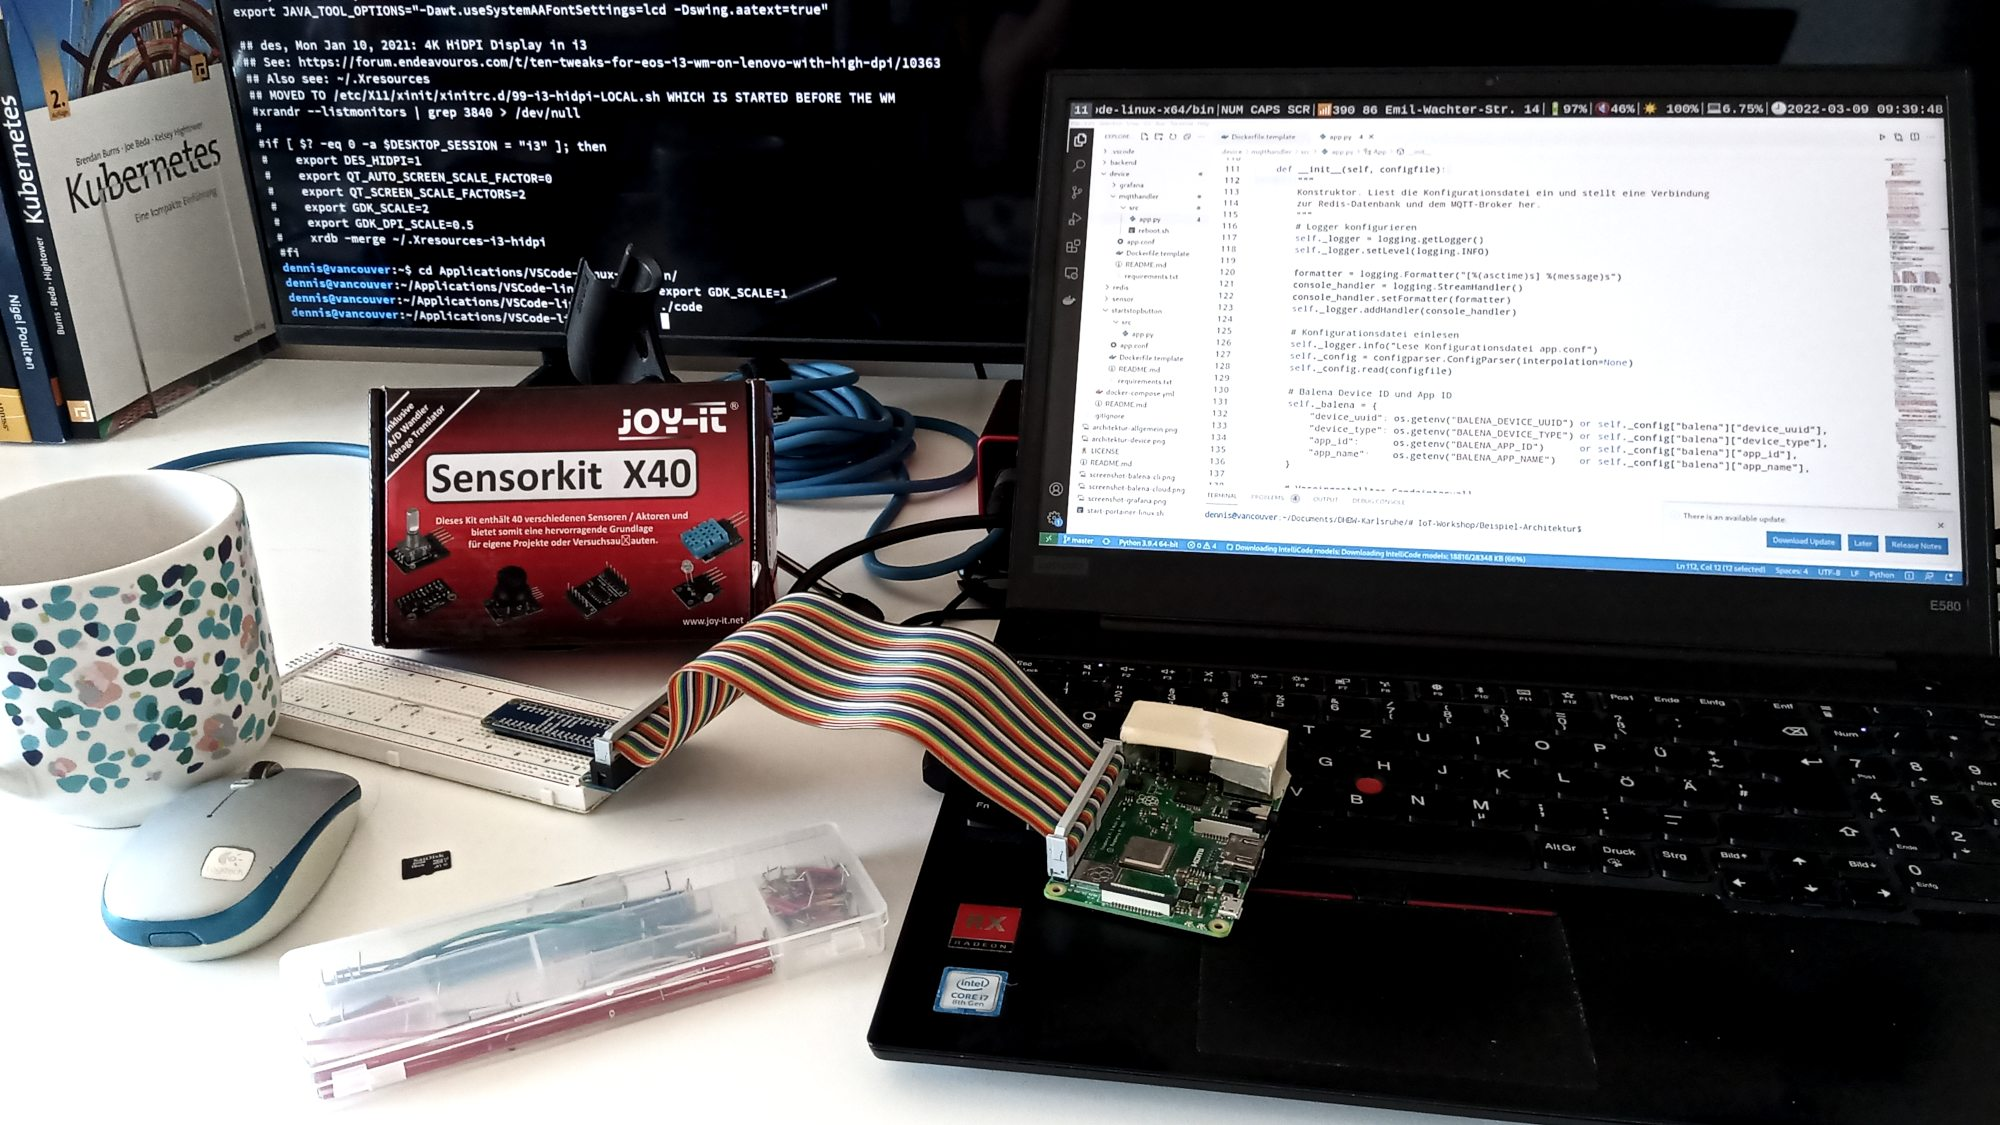
\includegraphics[width=\textwidth]{06-architektur/img/utensilien}
    \end{center}

    \footnotesize
    Laptop, Raspberry Pi, SD-Karte, Breadboard, Sensorkit, Kabel, Kaffee oder Tee
\end{frame}

%-------------------------------------------------------------------------------
\section{IoT-Entwicklung mit der Balena Cloud}
%-------------------------------------------------------------------------------

%%% Folie
{
\scriptsize

\begin{frame}{Anforderungen an die Systemarchitektur}

    \begin{columns}[T]
        \column{.3\textwidth}
        \begin{block}{Entwicklung}
            \smallskip
            Einfache Programmierung

            \smallskip
            Überschaubare Code-Struktur

            \smallskip
            Leichte Wartbarkeit

            \smallskip
            Nutzung von Bibliotheken

            \smallskip
            Nutzung des Betriebssystems

            \smallskip
            Schnelle Entwicklungszyklen
        \end{block}

        \column{.3\textwidth}
        \begin{block}{Betrieb}
            \smallskip
            Beliebig viele IoT-Devices

            \smallskip
            Unsichere Internetverbindung

            \smallskip
            Sensordaten zwischenspeichern

            \smallskip
            Neustart bei Stromausfall

            \smallskip
            Neustart bei Programmabstürzen

            \smallskip
            Protokollierung aller Aktionen
        \end{block}

        \column{.3\textwidth}
        \begin{block}{Steuerung}
            \smallskip
            Devices hinzufügen/entfernen

            \smallskip
            Einfache Überwachung

            \smallskip
            Konfiguration der Devices

            \smallskip
            Ausrollen von Updates

            \smallskip
            Fehlersuche auf den Devices

            \smallskip
            Hot Fix kritischer Fehler
        \end{block}
    \end{columns}

    \bigskip

    \begin{columns}[onlytextwidth]
        \column[b]{.33\textwidth}
        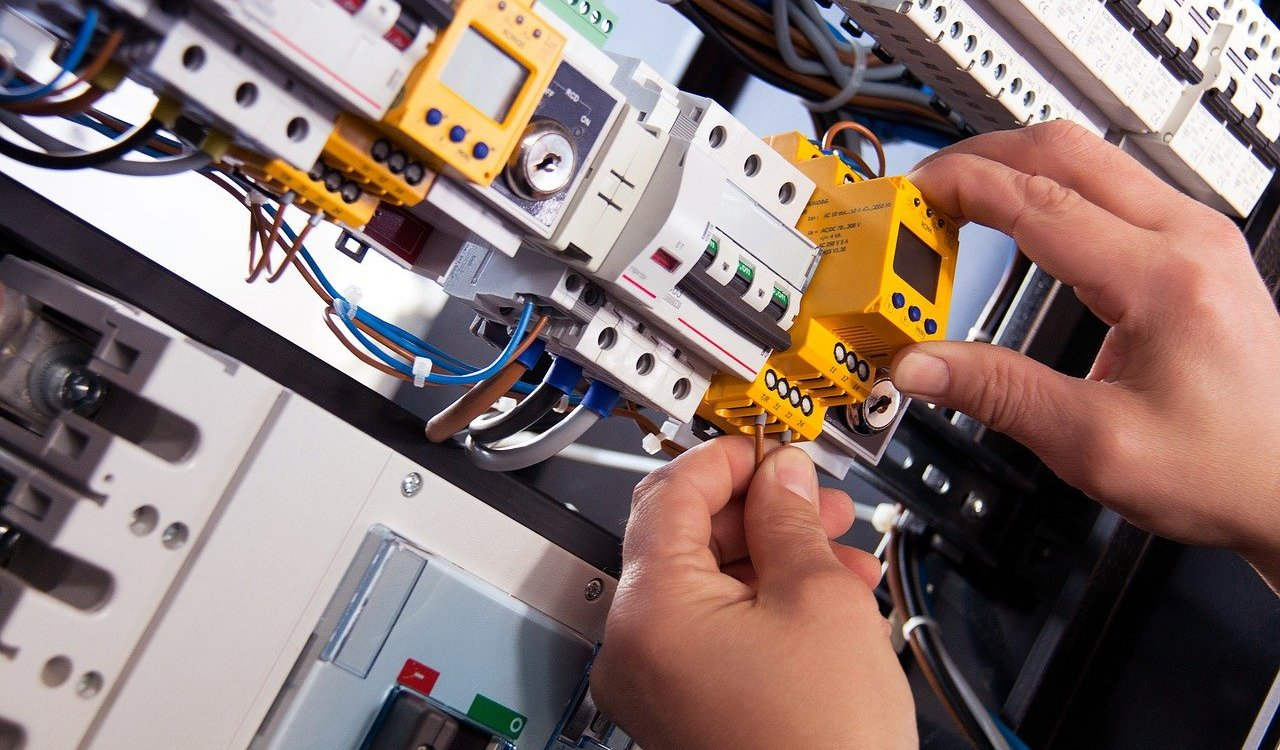
\includegraphics[width=\textwidth]{06-architektur/img/anforderungen1}

        \column[b]{.33\textwidth}
        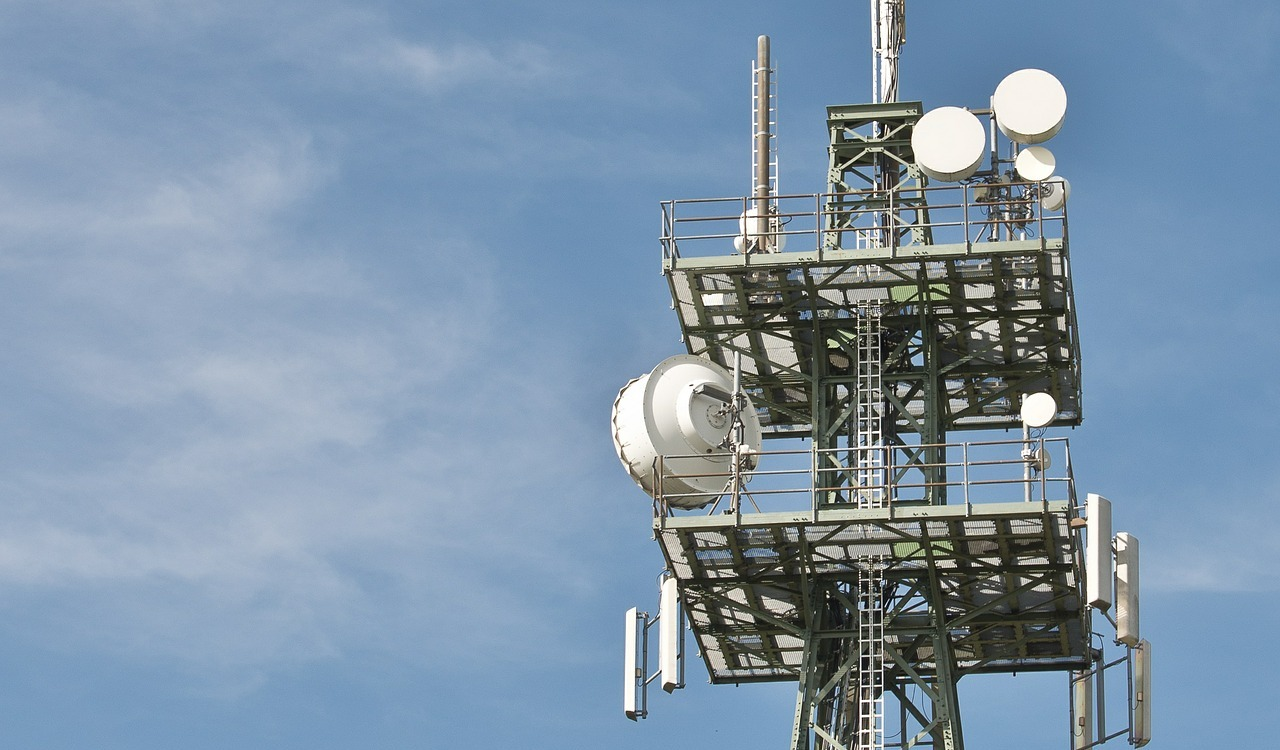
\includegraphics[width=\textwidth]{06-architektur/img/anforderungen2}

        \column[b]{.33\textwidth}
        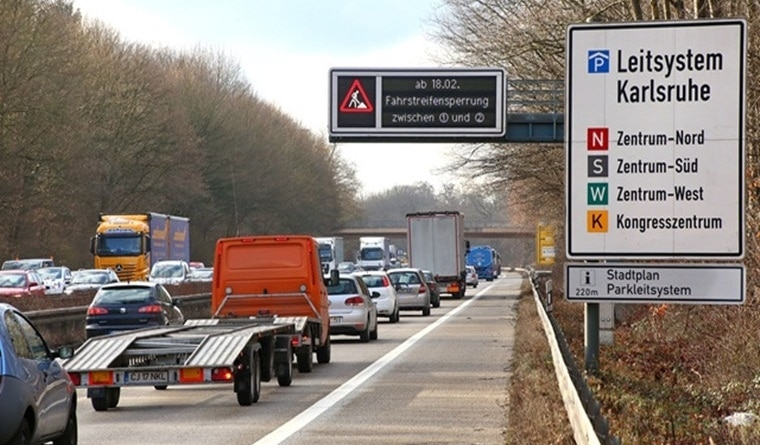
\includegraphics[width=\textwidth]{06-architektur/img/anforderungen3}
    \end{columns}

    \begin{columns}[onlytextwidth]
        \column[b]{.33\textwidth}
        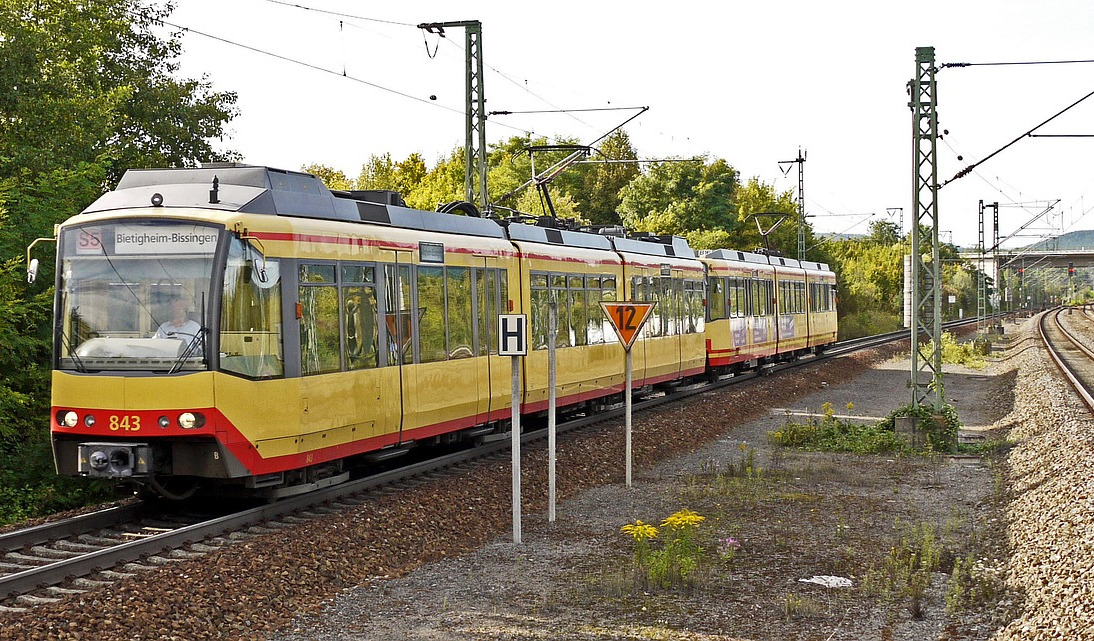
\includegraphics[width=\textwidth]{06-architektur/img/anforderungen4}

        \column[b]{.33\textwidth}
        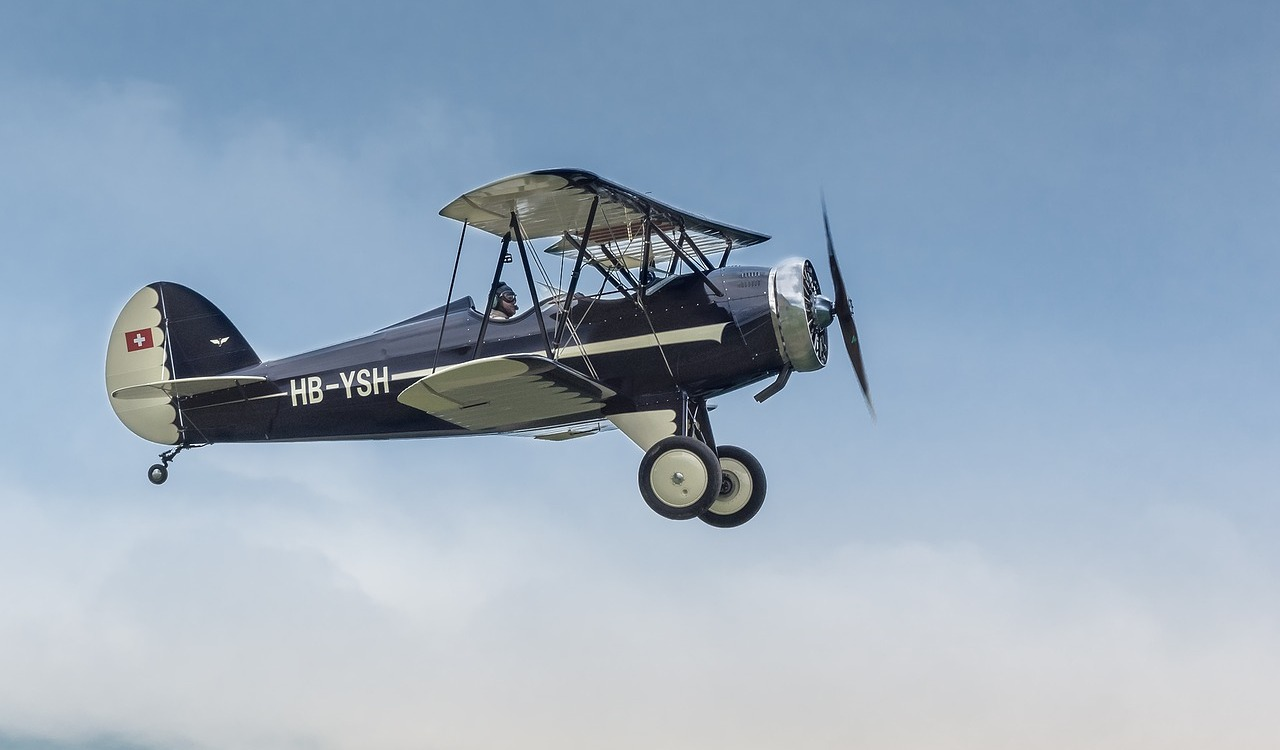
\includegraphics[width=\textwidth]{06-architektur/img/anforderungen5}

        \column[b]{.33\textwidth}
        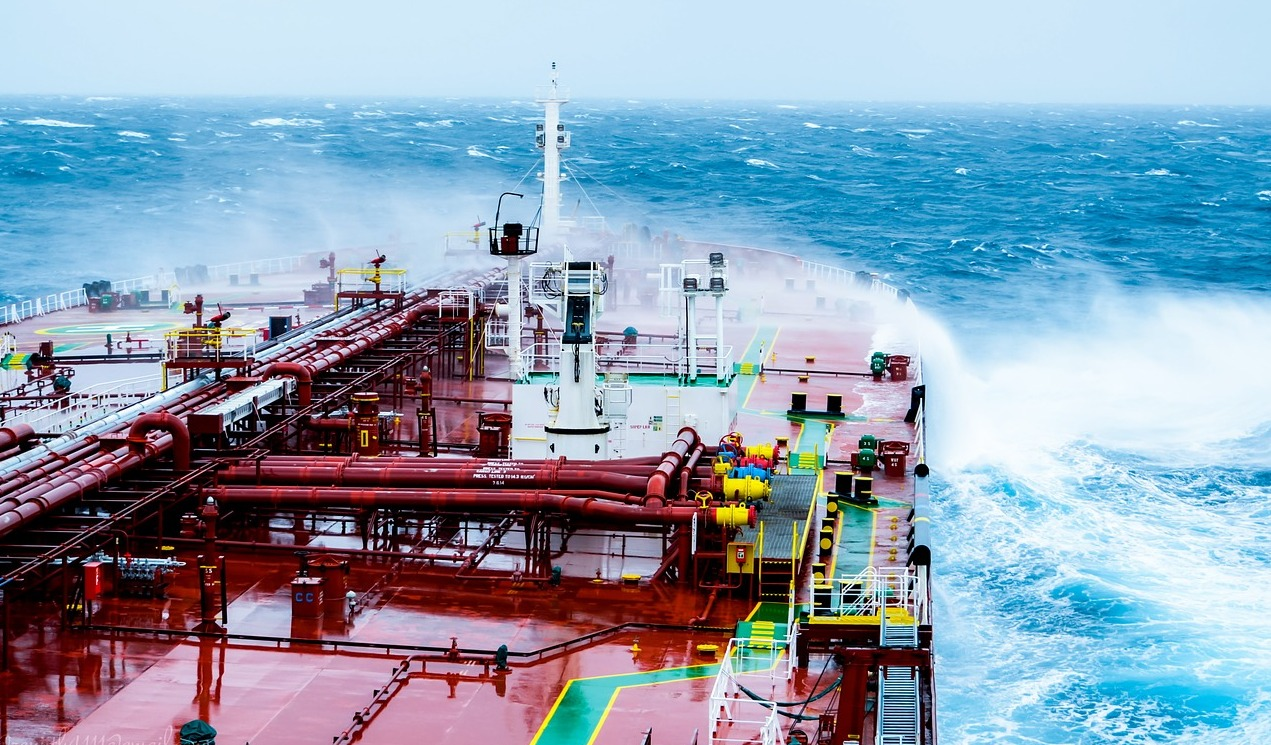
\includegraphics[width=\textwidth]{06-architektur/img/anforderungen6}
    \end{columns}
\end{frame}
}

%%% Folie
\begin{frame}{Remote Device Management mit Balena}
    \begin{center}
        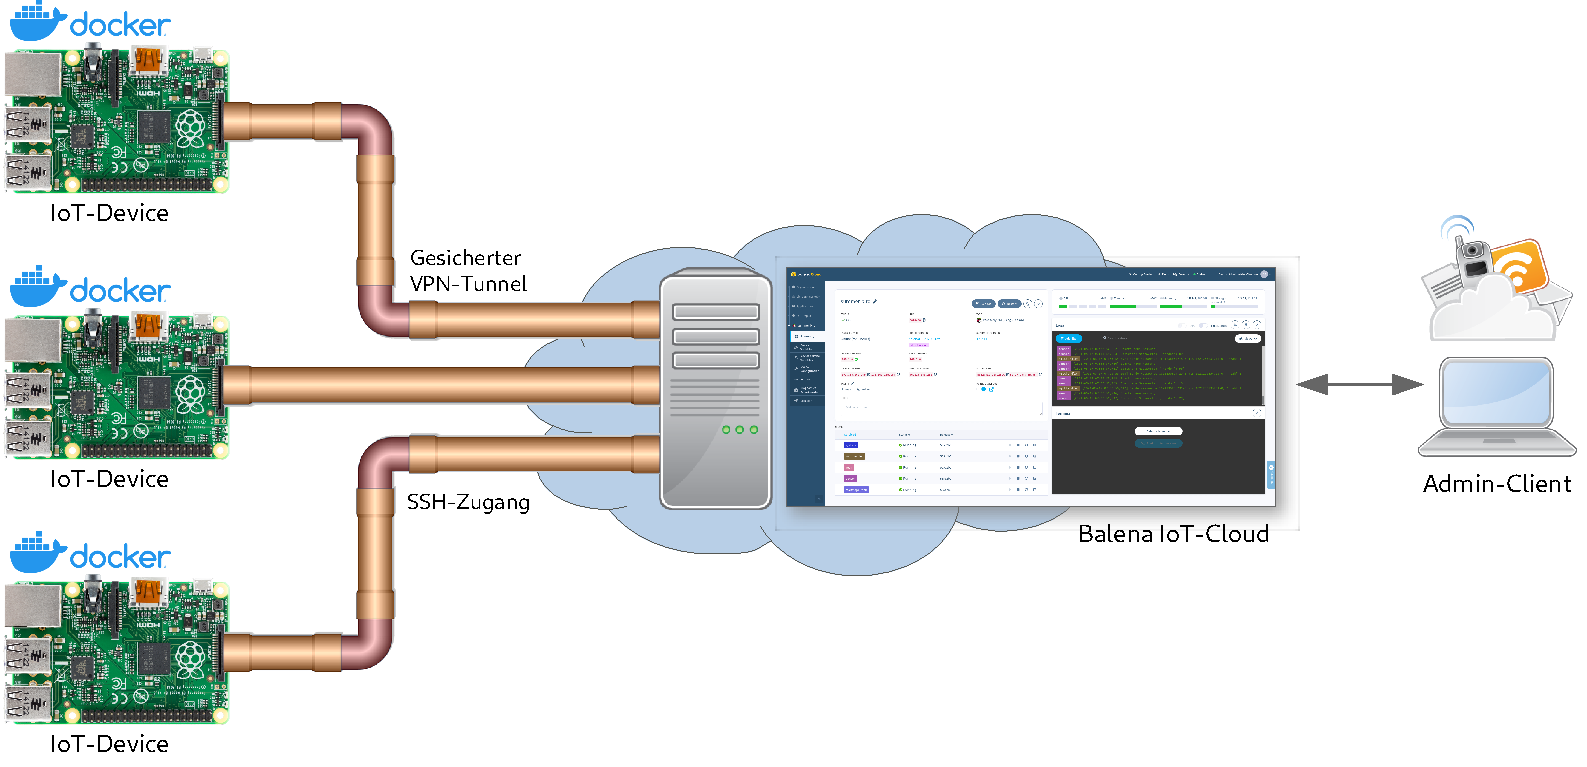
\includegraphics[width=\textwidth]{06-architektur/img/systemarchitektur1}
    \end{center}

    \Justified{
        \tiny
        Die \textbf{Balena IoT-Cloud} ermöglicht es, beliebig viele IoT-Devices
        zu einer IoT-Anwendung zusammenzufassen und die Devices hierfür mit
        einem \textbf{Linux-Betriebssystem} sowie darauf aufbauender Anwendungen
        zu provisionieren. Über einen gesicherten \textbf{VPN-Tunnel} sind die
        Devices mit der Cloud verbunden, so dass ihre Funktionsweise überwacht
        und vollautomatisiert Updates aufgespielt werden können.

        \smallskip
        Darüber hinaus können in der Cloud device-spezifische \textbf{Konfigurationswerte},
        die als Umgebungsvariablen des Betriebssystems im Quellcode zur Verfügung stehen,
        definiert werden.

        \smallskip
        Auf den Devices laufende \textbf{Serverdienste} können über eine
        \textbf{öffentliche URL} weltweit zugänglich gemacht werden.
    }
\end{frame}

%%% Folie
\begin{frame}{Internetkommunikation mit MQTT}
    \begin{center}
        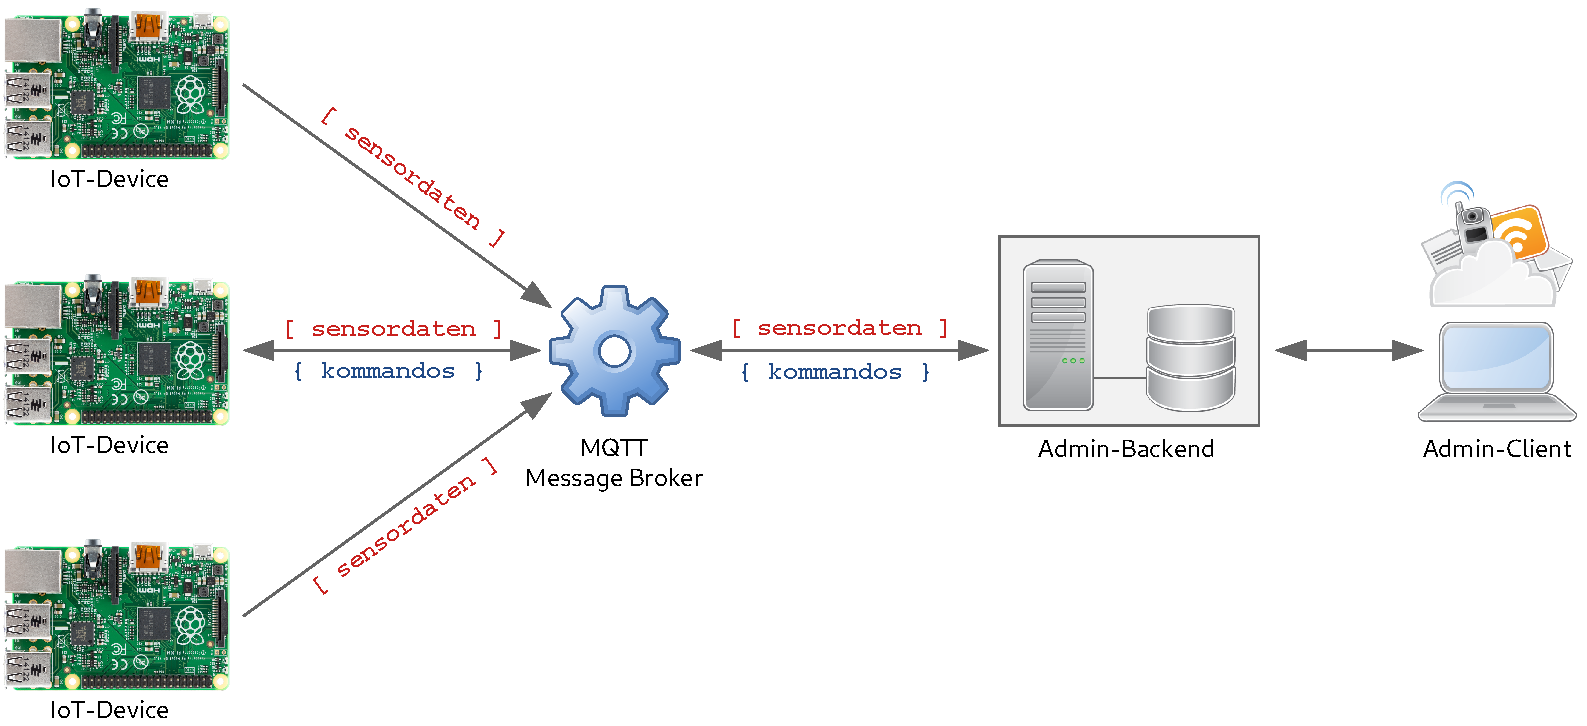
\includegraphics[width=\textwidth]{06-architektur/img/systemarchitektur2}
    \end{center}

    \smallskip

    \Justified{
        \tiny
        Die Kommunikation der Devices untereinander sowie mit dem Backend erfolgen
        über einen zentralen \textbf{MQTT Message Broker}. Dieser hat den Vorteil,
        dass den Devices (z.B. über Konfigurationswerte in der Balena Cloud) nur
        die Adresse des Brokers bekannt gemacht werden muss, um sie in die Anwendung
        zu integrieren.

        \smallskip
        Durch die Verwendung des \textbf{Publish/Subscribe}-Verfahrens mit
        unterschiedlichen Topics kann jede Komponente exakt die Daten empfangen,
        die sie benötigt. Derselbe Mechanismus kann daher nicht nur zum Versand
        von Sensordaten durch die Devices sondern auch zur Fernsteuerung der
        Devices mit anwendungsspezifischen Kommandos aus der Ferne genutzt werden.

        \smallskip
        Als Datenformat wird im Beispiel \textbf{UTF-8 kodiertes JSON} verwendet.
        Tatsächlich macht MQTT hierzu aber keine Vorgabe.
    }
\end{frame}

%%% Folie
\begin{frame}{Deviceseitige Integration mit Docker und Redis}
    \begin{center}
        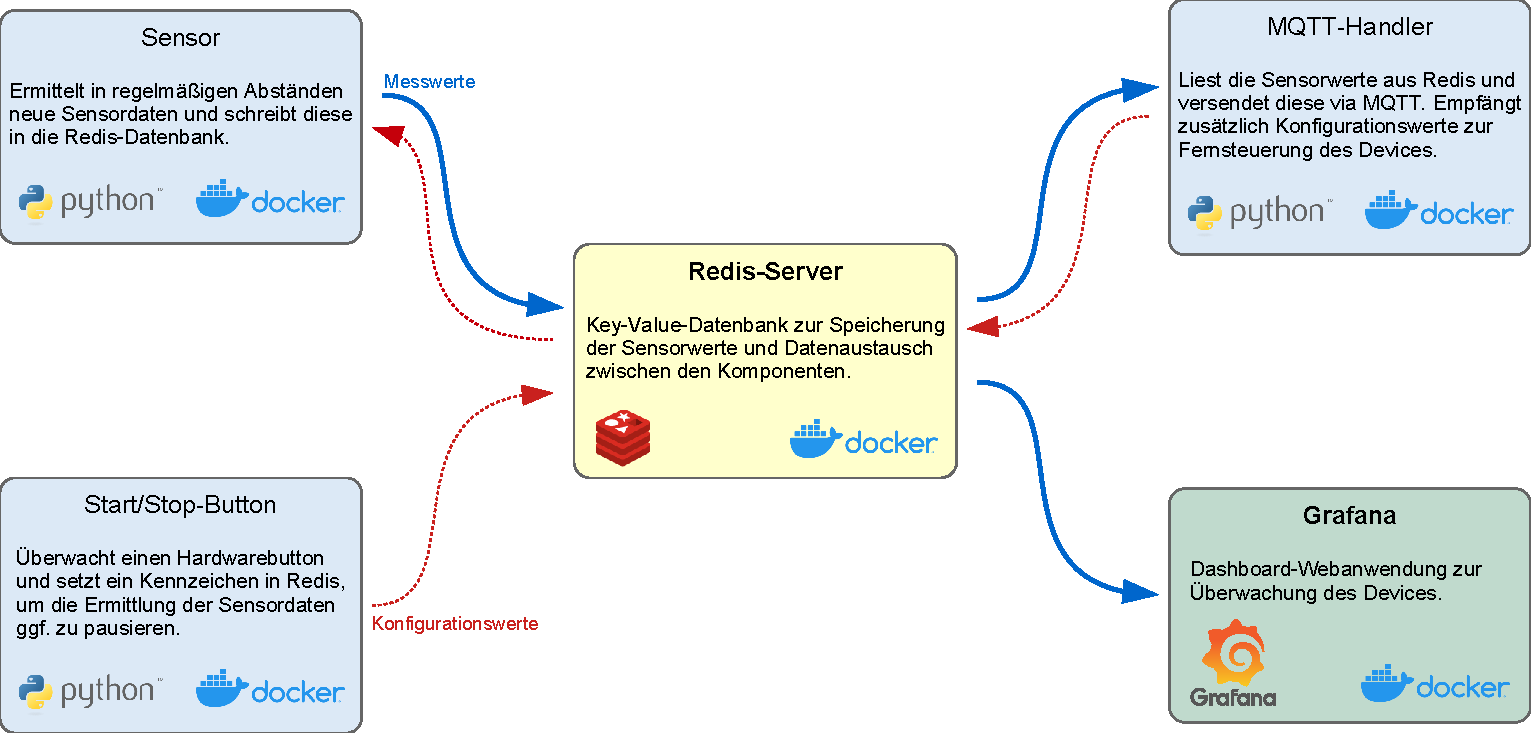
\includegraphics[width=\textwidth]{06-architektur/img/systemarchitektur3}
    \end{center}

    \smallskip

    \Justified{
        \tiny
        Die Verwendung von \textbf{Docker} zum Verpacken und Installieren der
        Anwendungen auf den Devices hat trotz des erhöhten Speicherbedarfs viele
        Vorteile. So kann über das \textbf{Docker Hub} auf eine große Bibliothek
        vorhandener Anwendungskomponenten wie z.B. \textbf{Redis} oder \textbf{Grafana}
        zurückgegriffen werden. Zusätzlich kann der deviceseitige Quellcode in
        kleine, eigenständige Programme zerlegt werden, um die Komplexität der
        Programmierung zu verringern und gleichzeitig die Ausfallsicherheit zu
        erhöhen.

        \smallskip
        Im gezeigten Beispiel dient \textbf{Redis} als zentraler Ablageort für
        Konfigurationswerte und zwischengespeicherte Sensordaten. Darüber hinaus
        erfolgt sämtliche Kommunikation zwischen den Teilanwendungen durch das
        Lesen und Schreiben von Daten in Redis. Hierfür können sich die Anwendungen
        eine Callback-Funktion registrieren, die bei Vorliegen neuer Daten in
        Redis automatisch aufgerufen wird.
    }
\end{frame}

%%% Folie
\begin{frame}{Generelle Vorgehensweise}
    \begin{adjustwidth}{-4ex}{-4ex}
        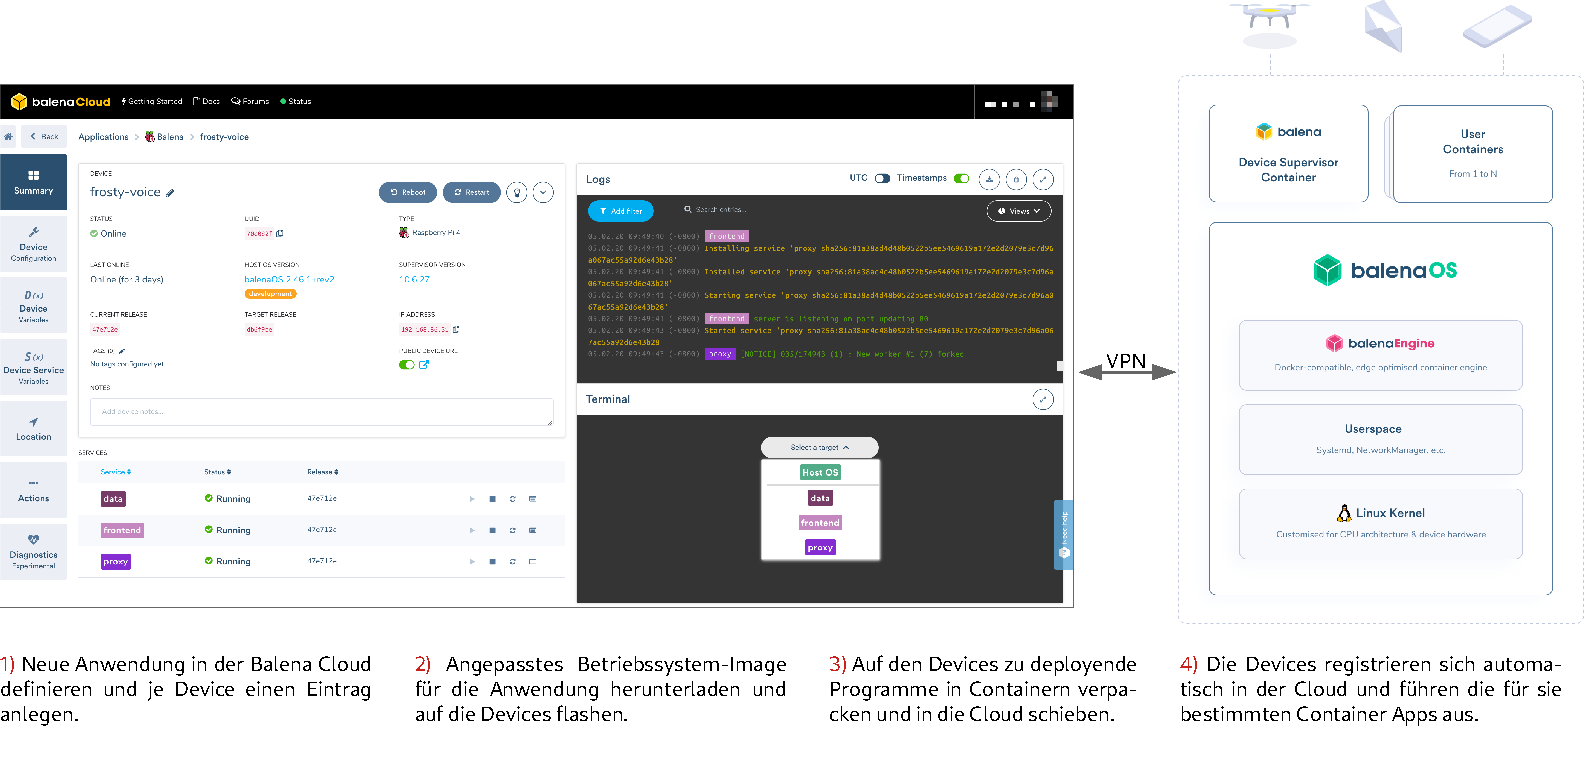
\includegraphics[width=\linewidth]{06-architektur/img/vorgehen}

        %\bigskip

        \Justified{
            \tiny
            Balena automatisiert nahezu alle Schritte von der Installation des
            Betriebssystems auf den Devices, dem Aufspielen der Quellcodes und
            Anwendungen sowie der Konfiguration und Überwachung der Devices.
            Hierfür muss lediglich eine neue Anwendung in der Balena Cloud
            registriert und für jede Geräteklasse ein Image des Balena OS
            konfiguriert und auf die Devices aufgespielt werden.

            \smallskip
            Die Devices verbinden sich nach dem Start automatisch über einen
            gesicherten VPN-Tunnel mit der Cloud und stellen sicher, dass
            sämtliche Anwendungskomponenten automatisch gestartet werden.
            Abstürzende Komponenten werden in der Regel ebenfalls einfach
            neugestartet.

            \smallskip
            Neue Softwareversionen werden automatisch auf die Devices
            ausgerollt. Dabei wird immer eine funktionierende Kopie des
            Betriebssystems und aller Anwendungen vorgehalten, so dass bei
            einem Installationsfehler automatisch auf die zuvor funktionierende
            Version umgeschaltet werden kann.
        }
    \end{adjustwidth}
\end{frame}

%%% Folie
\begin{frame}{Benötigte Entwicklungswerkzeuge}
    \begin{adjustwidth}{-4ex}{-4ex}
        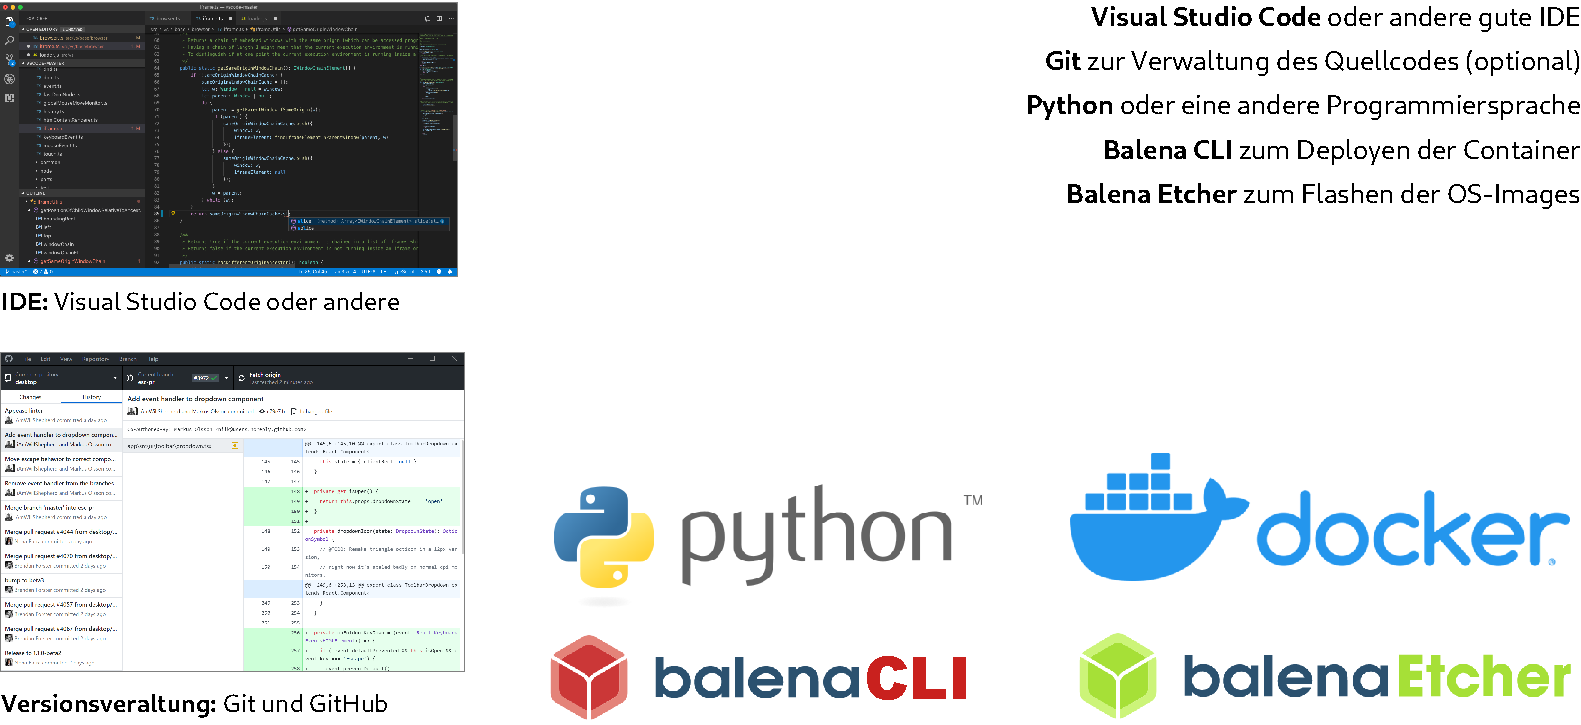
\includegraphics[width=\linewidth]{06-architektur/img/werkzeuge}

        \bigskip

        \Justified{
            \tiny
            Grundsätzlich werden für die Programmierung nicht viele Werkzeuge benötigt.
            Eine gute IDE mit integriertem Konsolenfenster (Terminal) wie \textbf{Visual
            Studio Code} sowie das \textbf{Balena CLI} (CLI = Command Line Interface)
            genügen im Grunde genommen schon. Mit \textbf{Balena Etcher} steht darüber
            hinaus ein einfach zu bedienendes Programm zum Aufspielen von Filesystem
            Images auf die SD-Karte des Raspberry Pi zur Verfügung.

            \smallskip
            In größeren Projekten bietet es sich darüber hinaus an, den Quellcode
            mit Git zu versionieren und z.B. über GitHub zu teilen. Zusätzlich kann
            Docker auch lokal verwendet werden, um Backendstrukturen wie Datenbanken,
            Admin-Oberflächen, Dashboards usw. lokal zu entwickeln und zu testen.
        }
    \end{adjustwidth}
\end{frame}

%%% Folie
{
\footnotesize

\begin{frame}{Link zum Quellcode}
    \url{https://github.com/DennisSchulmeister/dhbwka-wwi-iotws-architektur}

    \smallskip
    \setlength{\fboxsep}{0em}
    \fbox{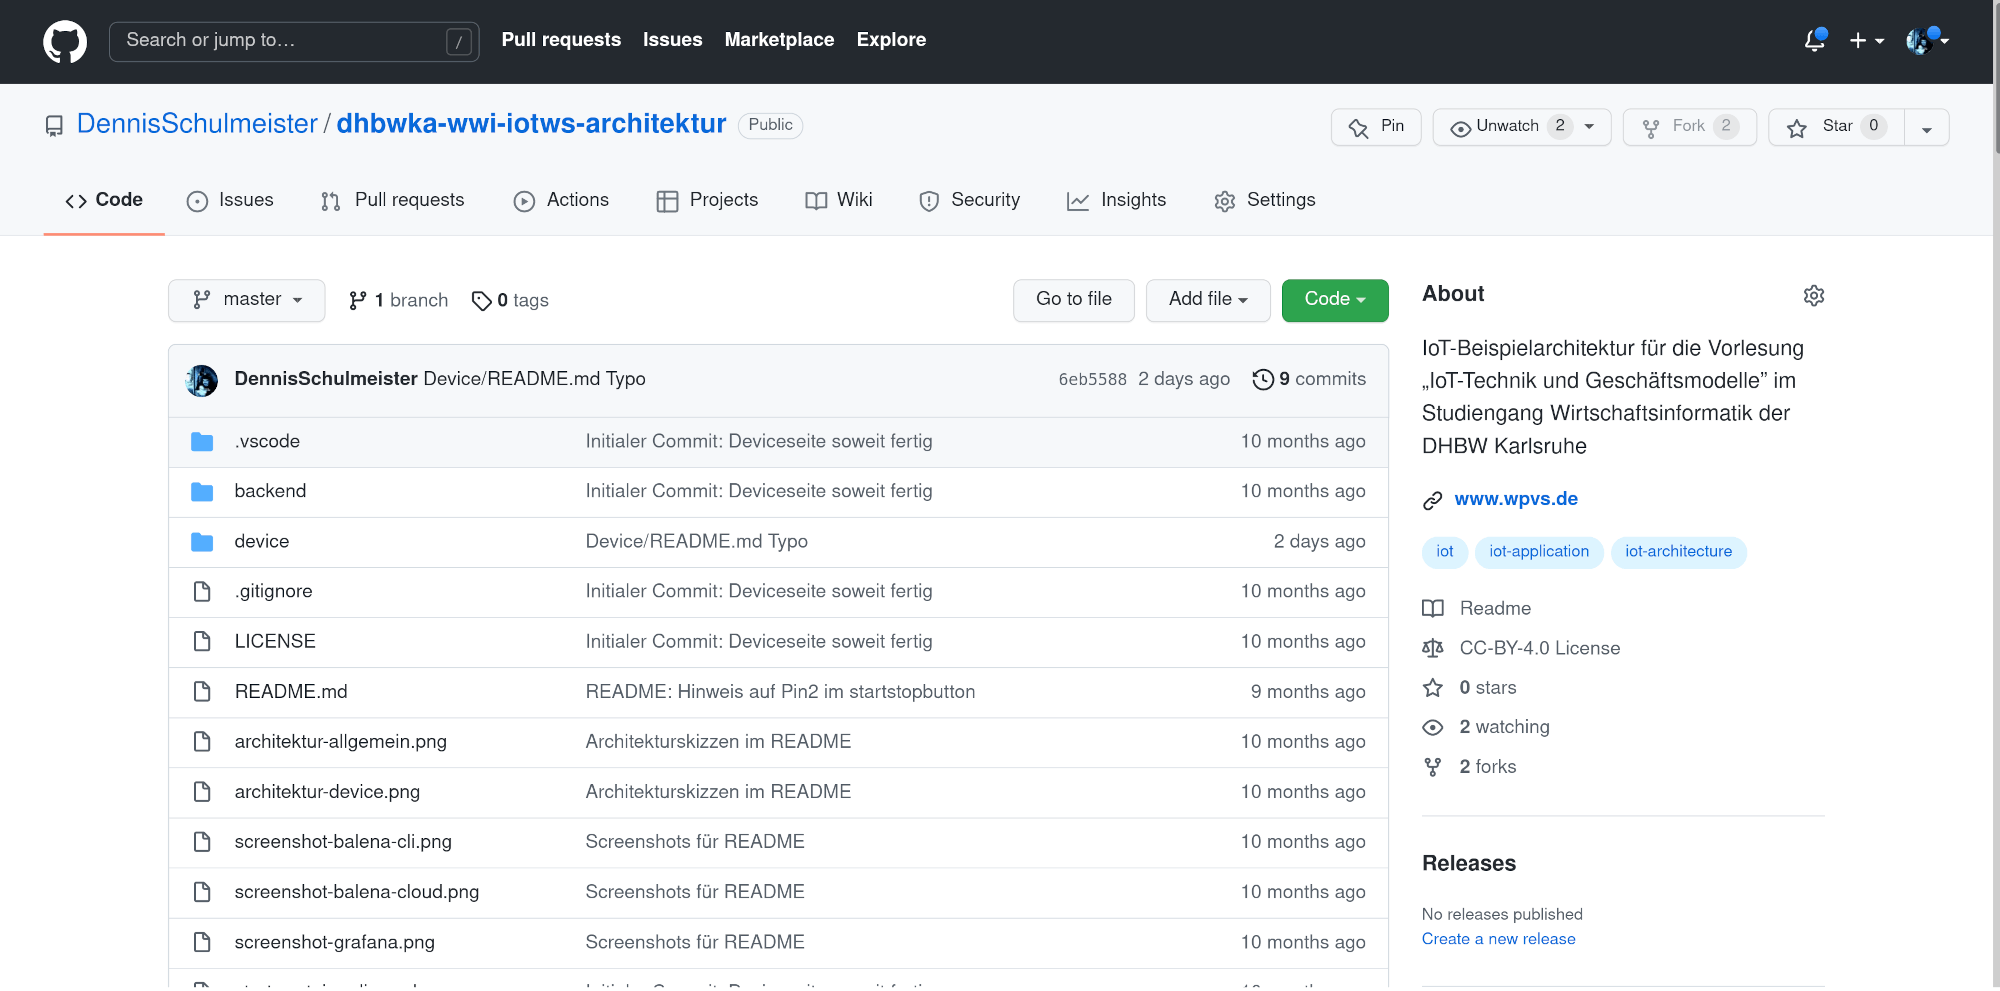
\includegraphics[width=\textwidth]{06-architektur/img/github}}
\end{frame}
}

%%% Folie
{
\small

\begin{frame}{Aufgabe: Let's get started}
    \begin{enumerate}
        \item Legen Sie einen Test Account in der Balena Cloud an.
        \item Registrieren Sie eine neue Anwendung für unsere Vorlesung.
        \item Konfigurieren Sie das Balena OS und spielen es auf den Rasbperry Pi auf.
        \item Laden Sie sich den Quellcode der Beispielanwendung herunter.
        \item Deployen Sie den Beispielquellcode zunächst im Produktivmodus auf dem Pi.
        \item Aktivieren Sie anschließend den Live-Entwicklungsmodus.
        \item Nehmen Sie eine Änderung am Quellcode vor und testen diesen auf dem Pi.
    \end{enumerate}
\end{frame}
}

%%% Folie
{
\scriptsize

\begin{frame}{Was ist Docker?}
    \Justified{
        Docker ist eine \textbf{Laufzeitumgebung zur Isolation laufender Prozesse}
        unter Linux. (Aktuelle Versionen von Microsoft Windows unterstützen diese
        Funktion inzwischen auch). Die Programme werden hierfür mit allen für ihre
        Ausführung benötigten Systembibliotheken und Hilfsdateien in binäre Filesystem
        Images (hier \textbf{Container Image} genannt) verpackt und dann durch den
        Docker Daemon also sog. \textbf{Container} ausgeführt, wobei das Wort
        Container hier die Isolation der Prozesse verdeutlichen soll.

        \smallskip
        Intern werden hierfür verschiedene Mechanismen des Linux-Kernels genutzt,
        um den Programmen vorzugaukeln, dass sie die einzigen laufenden Programme
        innerhalb des Betriebssystems wären. Gute Container Images starten daher
        tatsächlich nur einen Prozess, der automatisch die \textbf{Prozess-ID 1}
        bekommt.

        \smallskip
        Darüber hinaus virtualisiert Docker das Netzwerk sowie den Massenspeicher,
        um die Container noch weiter voneinander zu isolieren. Zusammengehörige
        Container können über ein \textbf{virtuelles Netzwerk} untereinander
        kommunizieren und einzelne Ports können vom Host an die Container
        weitergeleitet werden.

        \smallskip
        Wichtig zu verstehen ist, dass Container ,,immutabel'' sind, was bedeutet,
        dass sie zwar Dateien in ihrem virtuellen Dateisystem erzeugen können,
        diese bei einem Neustart des Containers aber verloren gehen. Über sog.
        \textbf{Volumes} können stattdessen externe Massenspeicher angebunden
        werden, um persistente Daten abzulegen.
    }

    \bigskip

    \begin{columns}[onlytextwidth]
        \column[b]{.49\textwidth}
        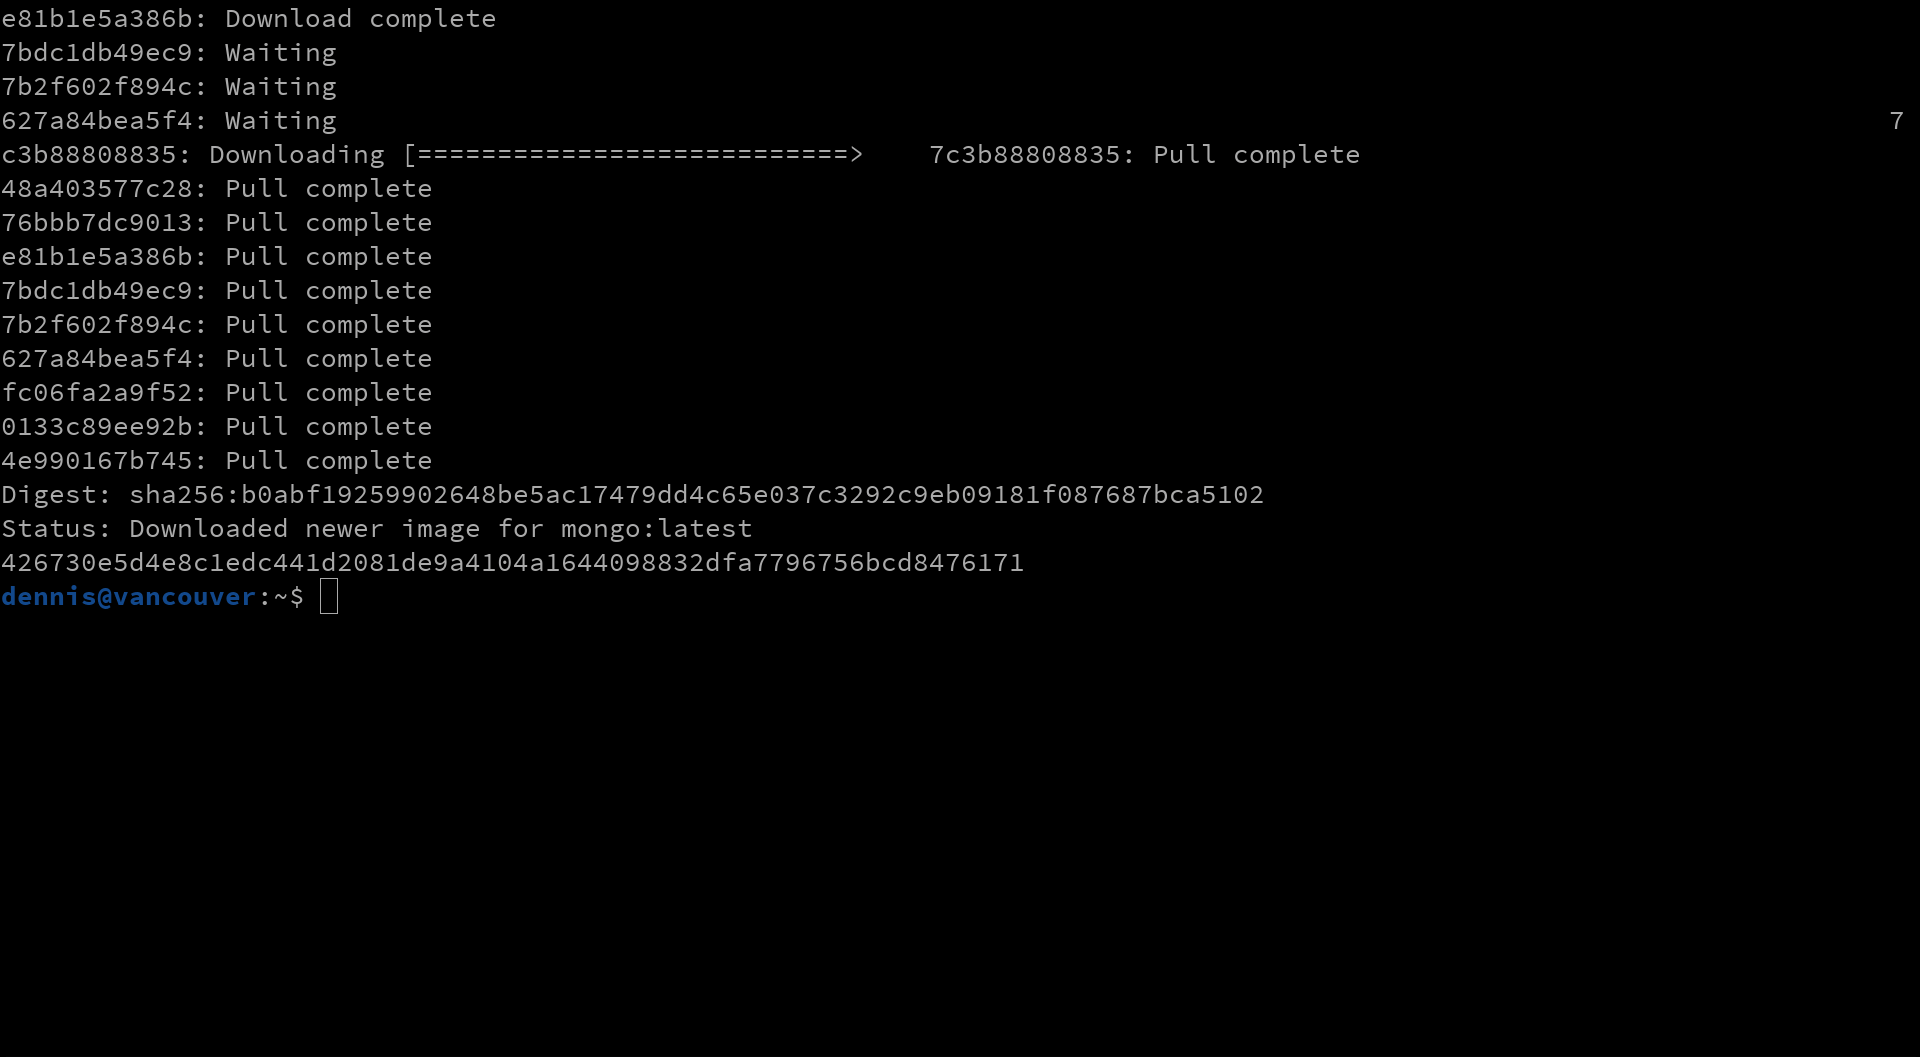
\includegraphics[width=\textwidth]{06-architektur/img/docker1}

        \column[b]{.49\textwidth}
        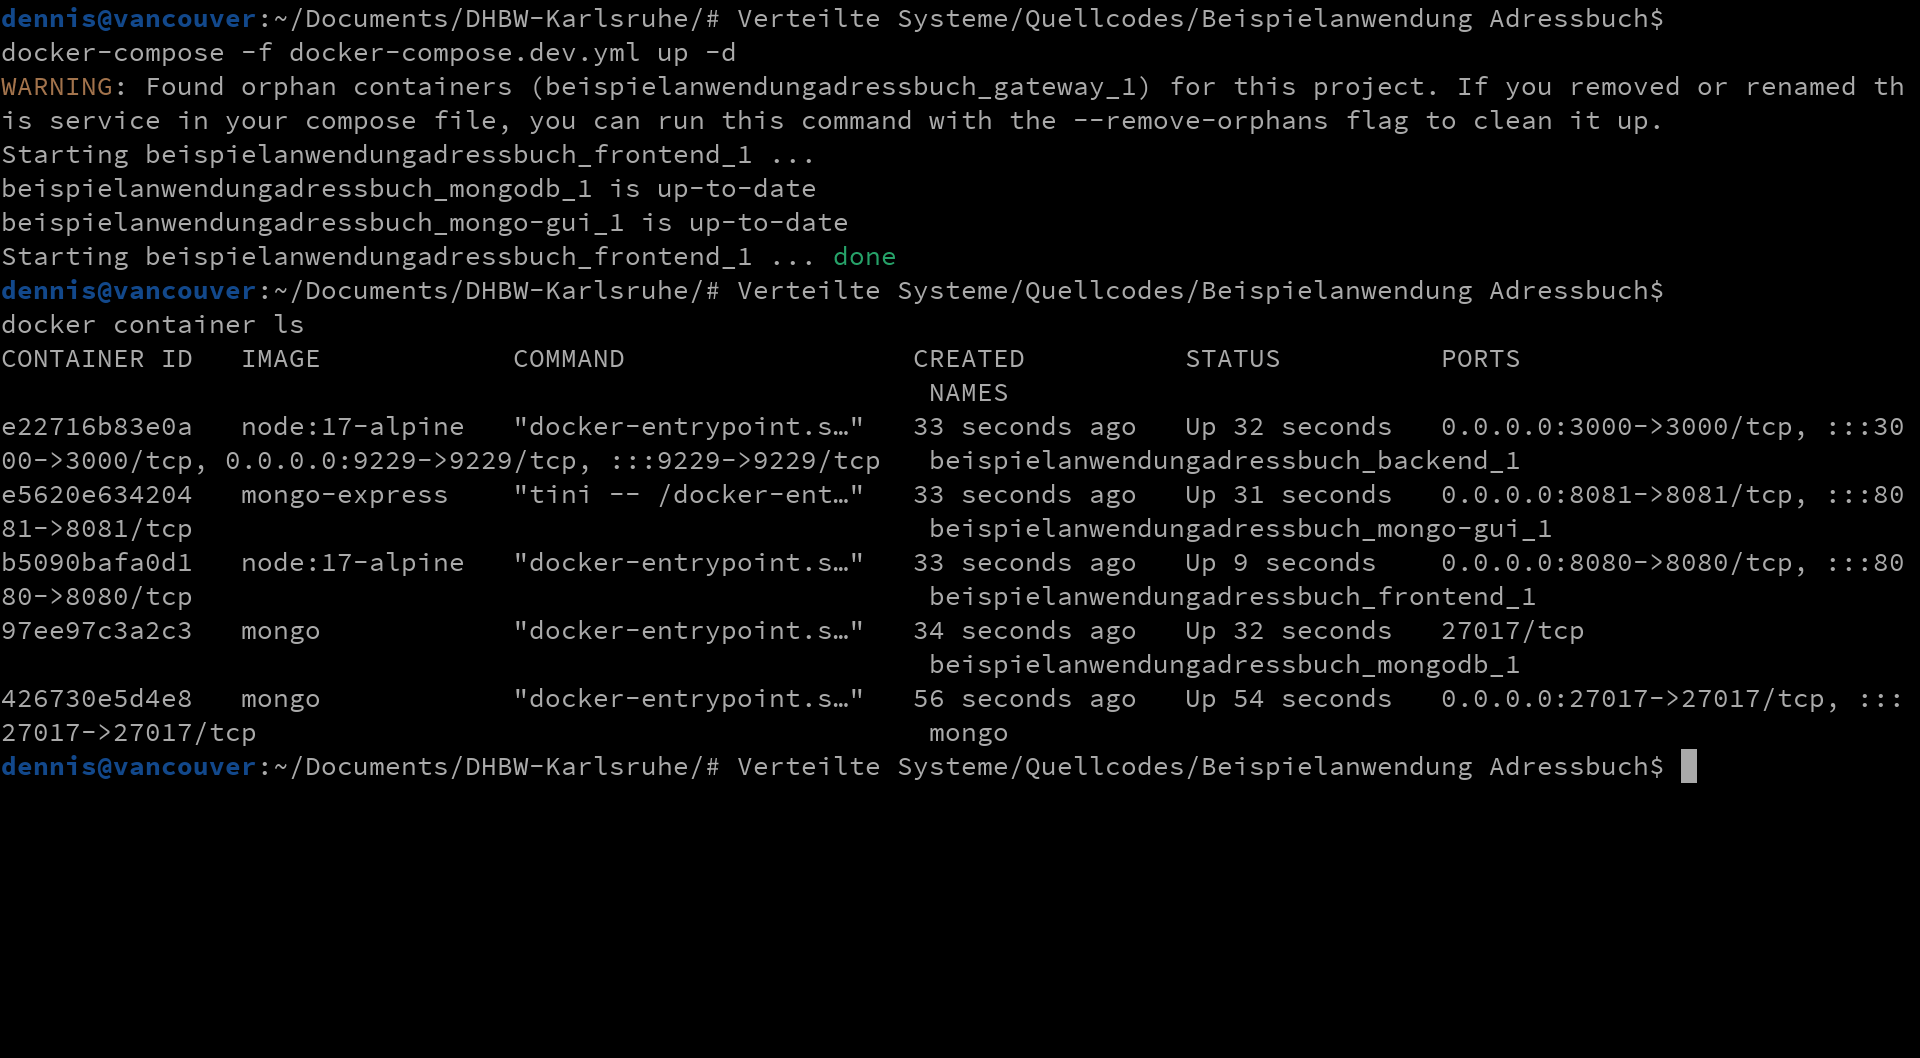
\includegraphics[width=\textwidth]{06-architektur/img/docker2}
    \end{columns}
\end{frame}
}

%%% Folie
{
\scriptsize

\begin{frame}{Unterschied zur Vollvirtualisierung}
    \begin{adjustwidth}{-4ex}{-4ex}
        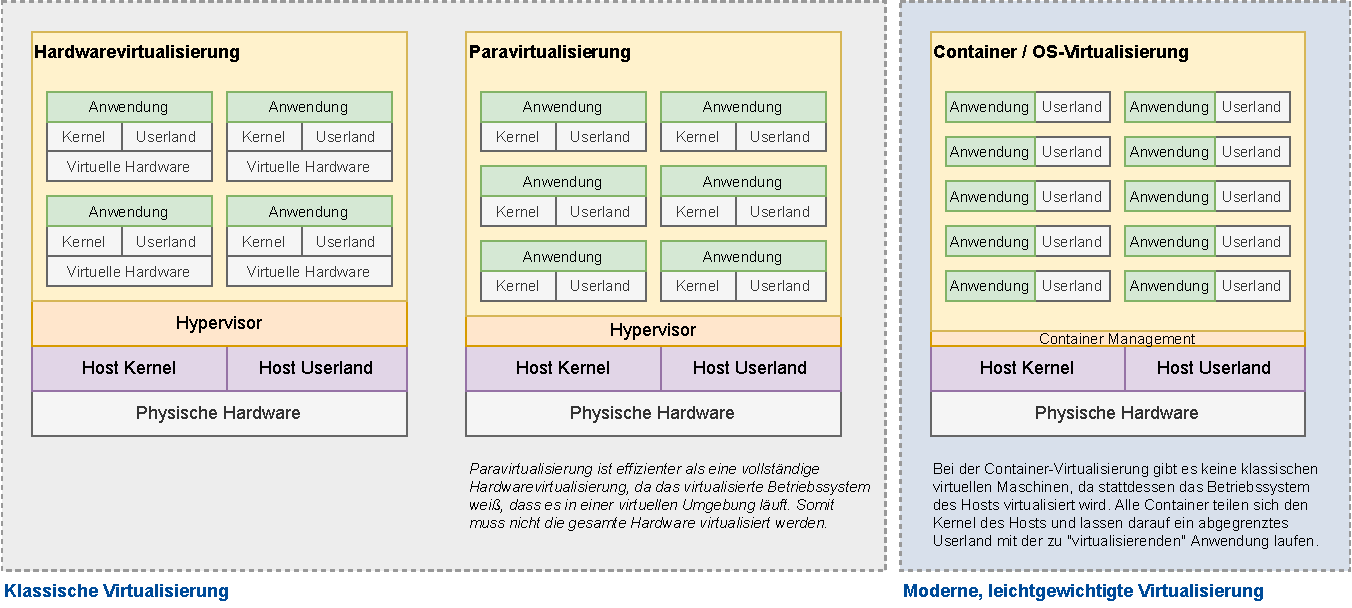
\includegraphics[width=\linewidth]{06-architektur/img/docker-virtualisierung}

        \bigskip

        \Justified{
            Docker realisiert eine Quasi-Virtualisierung, indem den in den Containern
            laufenden Programmen vorgegaukelt wird, dass sie die einzigen Programme
            des Host-Betriebssystems seien. Dadurch entsteht im Vergleich zu richtiger
            Hardwarevirtualisierung ein kaum merkbarer Verwaltungsoverhead. Jedoch
            belegen Docker Container unter Umständen mehr Speicher als es die Programme
            ohne Docker tun würden, jedoch weit weniger Speicher als bei der klassischen
            Virtualisierung (da nur ein Rumpf-Betriebssystem mitgeliefert werden muss).
        }
    \end{adjustwidth}
\end{frame}
}

%%% Folie
{
\scriptsize

\begin{frame}{Container Images mit einem Dockerfile}
    \Justified{
        Um ein sog. Image zu bauen, das von Docker als Container ausgeführt werden
        kann, muss im Quellcode-Verzeichnis des Programms eine Datei namens
        \texttt{Dockerfile} angelegt werden. Ihre Aufgabe ist zu beschreiben,
        aus welchen Inhalten (also aus welchen Dateien) sich das Image zusammensetzen
        soll. Hierfür wird in der Regel aus dem \textbf{Docker Hub} (allgemein auch
        ,,Registry'' genannt) ein vorhandenes Image referenziert und um eigene
        Dateien erweitert. Als Basis-Image kann dann entweder ein minimales
        Betriebssystem-Image (z.B. Debian oder Alpine Linux) oder eine
        vorkonfigurierte Laufzeitumgebung wie Node.js, Python, … (die selbst auf
        einem der genannten Betriebssystem-Images basiert) ausgewählt werden.
    }

    \bigskip

    {
    \tiny
    \arrayrulecolor{gray}

    \begin{tabular}{|p{\textwidth}|}
        \hline

        \cellcolor{gray!15}
        \texttt{\textbf{FROM} balenalib/\%\%BALENA\_MACHINE\_NAME\%\%-debian-python:latest-run} \\
        \cellcolor{gray!15}
        \textcolor{darkgray}{Referenzierung des Basis-Containers (mit Balena-Platzhalter für die CPU-Architektur)} \\

        \cellcolor{gray!7}
        \\

        \cellcolor{gray!15}
        \texttt{\textbf{RUN} apt-get -y update; apt-get -y upgrade; apt-get -y install build-essential} \\
        \cellcolor{gray!15}
        \textcolor{darkgray}{Ausführung eines Befehls zur Installation weiterer Pakete im Container Image} \\
        \cellcolor{gray!15}
        \textcolor{darkgray}{(Workaround, damit RPi.GPIO während der Installation kompiliert werden kann)} \\

        \cellcolor{gray!7}
        \\

        \cellcolor{gray!15}
        \texttt{\textbf{WORKDIR} /usr/src/app} \\
        \cellcolor{gray!15}
        \textcolor{darkgray}{Wechseln des für die folgenden Befehle verwendeten Arbeitsverzeichnisses im Image} \\

        \cellcolor{gray!15}
        \texttt{\textbf{COPY} requirements.txt .} \\
        \cellcolor{gray!15}
        \textcolor{darkgray}{Datei \texttt{requirements.txt} in das eben ausgewählte Arbeitsverzeichnis kopieren} \\

        \cellcolor{gray!15}
        \texttt{\textbf{RUN} pip install --no-cache-dir -r requirements.txt} \\
        \cellcolor{gray!15}
        \textcolor{darkgray}{Ausführung eines Befehls, um die benötigten Python-Bibliotheken zu installieren} \\

        \cellcolor{gray!7}
        \\

        \cellcolor{gray!15}
        \texttt{\textbf{COPY} app.conf .} \\
        \cellcolor{gray!15}
        \textcolor{darkgray}{Datei \texttt{app.conf} in das eben ausgewählte Arbeitsverzeichnis kopieren} \\

        \cellcolor{gray!15}
        \texttt{\textbf{COPY} ./src .} \\
        \cellcolor{gray!15}
        \textcolor{darkgray}{Zum Schluss den eigentlichen Quellcode in das Filesystem Image kopieren} \\

        \cellcolor{gray!7}
        \\

        \cellcolor{gray!15}
        \texttt{\textbf{ENTRYPOINT} ["python", "app.py"]} \\
        \cellcolor{gray!15}
        \textcolor{darkgray}{Definition des zur Ausführung des Containers zu startenden Programms} \\
        \hline
    \end{tabular}
    }
\end{frame}
}

%%% Folie
{
\scriptsize

\begin{frame}[fragile]{Container orchestrieren mit Docker Compose}
    \Justified{
        Da die Befehlsketten zur Ausführung und Verknüpfung mehrerer Docker-Container
        mitunter sehr komplex werden können, lässt sich ein Setup aus zusammenhängenden
        Containern auch deklarativ in einer Datei namens \texttt{docker-compose.yml}
        beschreiben. Das Werkzeug \textbf{Docker Compose} übernimmt dann den Start
        und auch die Beendigung aller Container in der richtigen Reihenfolge.
        Außerdem kann damit eine einfache Skalierung durch Starten mehrerer,
        paralleler Containerinstanzen erreicht werden.
    }

    \begin{lstlisting}[language={}, gobble=8, basicstyle=\tiny\ttfamily]
        version: '2'

        volumes:
            redis-data:

        services:
            # Redis Key-Value Store
            redis:
                build: redis/
                restart: always
                volumes:
                    - 'redis-data:/data'
                expose:
                    - 6379

            # Programm zum Auslesen der Sensordaten
            sensor:
                build: sensor/
                privileged: true
                restart: always
                depends_on:
                    - redis
                environment:
                    - REDIS_HOST=redis
                    - REDIS_PORT=6379
                    - REDIS_DB=0

            ...
    \end{lstlisting}
\end{frame}
}

%%% Folie
{
\small

\begin{frame}{Aufgabe: Verwendung von Docker}
    \begin{enumerate}
        \item Welche Schritte führen die Dockerfiles im Beispielquellcode aus?
        \item Entfernen Sie das Grafana Dashboard von den Devices.
        \item Fügen Sie stattdessen \texttt{docker/getting-started} hinzu.
        \item Machen Sie Port 80 des Getting-Started-Services öffentlich zugänglich.
        \item Entfernen Sie anschließend den Getting-Started-Service wieder.
    \end{enumerate}
\end{frame}
}

%-------------------------------------------------------------------------------
\section{Nutzung des Redis Key-Value-Store}
%-------------------------------------------------------------------------------

%%% Folie
\begin{frame}{Was ist Redis?}
    \begin{center}
        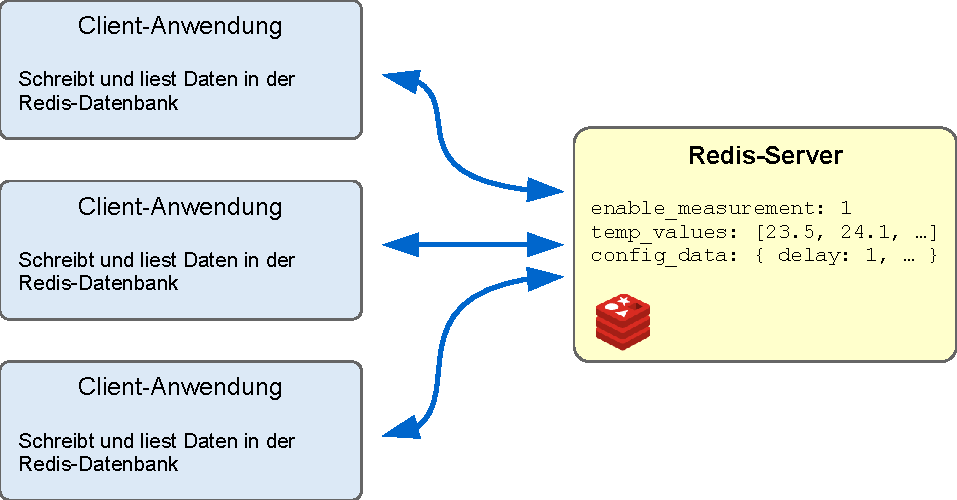
\includegraphics[width=.8\textwidth]{06-architektur/img/redis1}
    \end{center}

    \Justified{
        \tiny
        Redis ist eine NoSQL-Datenbank nach dem Prinzip eines \textbf{Key-Value-Servers}.
        Anders als die meisten Datenbanken konzentriert sich Redis nicht darauf, große
        Mengen an mehr oder weniger strukturierten Daten zu persistieren, sondern eine
        kleine Auswahl \textbf{flexibel einsetzbarer Datenstrukturen} im Speicher halten
        zu können. Die Datenstrukturen entsprechen im Wesentlichen denselben Strukturtypen,
        wie sie auch aus anderen Hochsprachen wir Python oder JavaScript bekannt sind:

        \begin{itemize}
            \setlength\itemsep{.5em}
            \item Binärstrings
            \item Listen
            \item (Un)sortierte Mengen
            \item Hashes / Dictionaries
            \item Bit-Arrays
            \item Streams
        \end{itemize}
    }
\end{frame}

%%% Folie
\begin{frame}{Performance vs. Persistenz in Redis}
    \begin{center}
        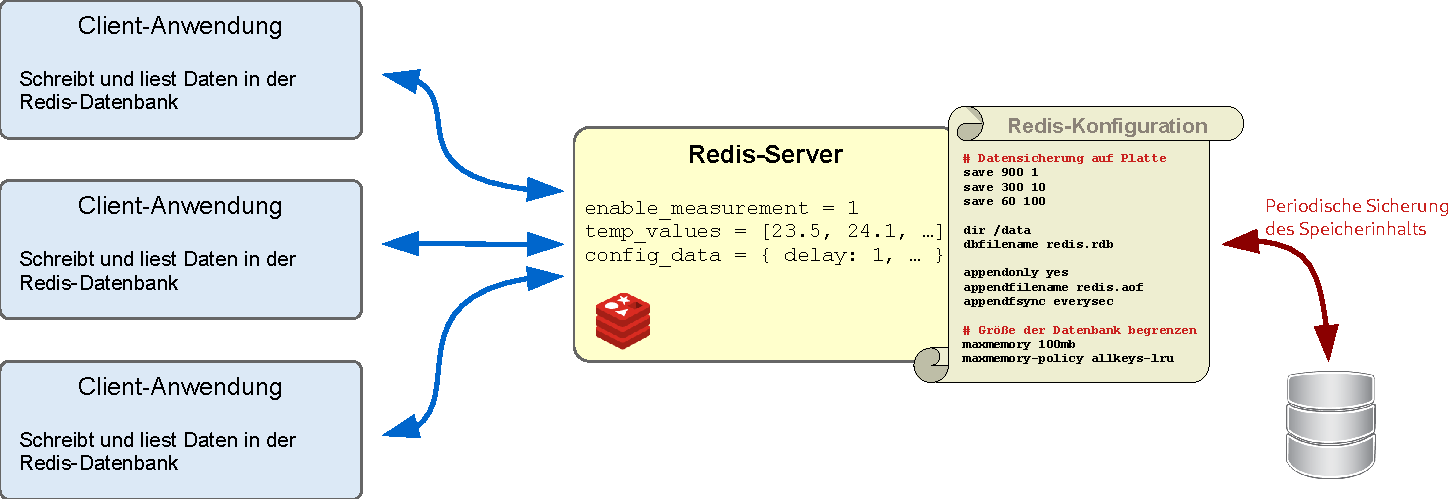
\includegraphics[width=\textwidth]{06-architektur/img/redis2}
    \end{center}

    \bigskip

    \Justified{
        \scriptsize
        Grundsätzlich hält Redis sämtliche Daten im Hauptspeicher vor (sog.
        \textbf{In-Memory-Database}). Datenzugriffe erfolgen daher sehr schnell,
        da die Daten niemals von langsamen Massenspeichern gelesen werden müssen.
        Dennoch werden die Daten in konfigurierbaren Intervallen bei Vorliegen
        von genügend vielen Änderungen oder Ablauf vorgegebener Fristen in ein
        Journal auf Platte geschrieben, damit sie nicht verloren gehen. Beim Start
        des Servers wird das Journal dann wieder in den Hauptspeicher geladen.
        Zusätzlich kann die maximale Speicherbelegen limitiert werden, um somit
        einen effizienten Ringspeicher zu realisieren.
    }
\end{frame}

%%% Folie
\begin{frame}{Verwendung von Redis in der Beispielarchitektur}
    \begin{center}
        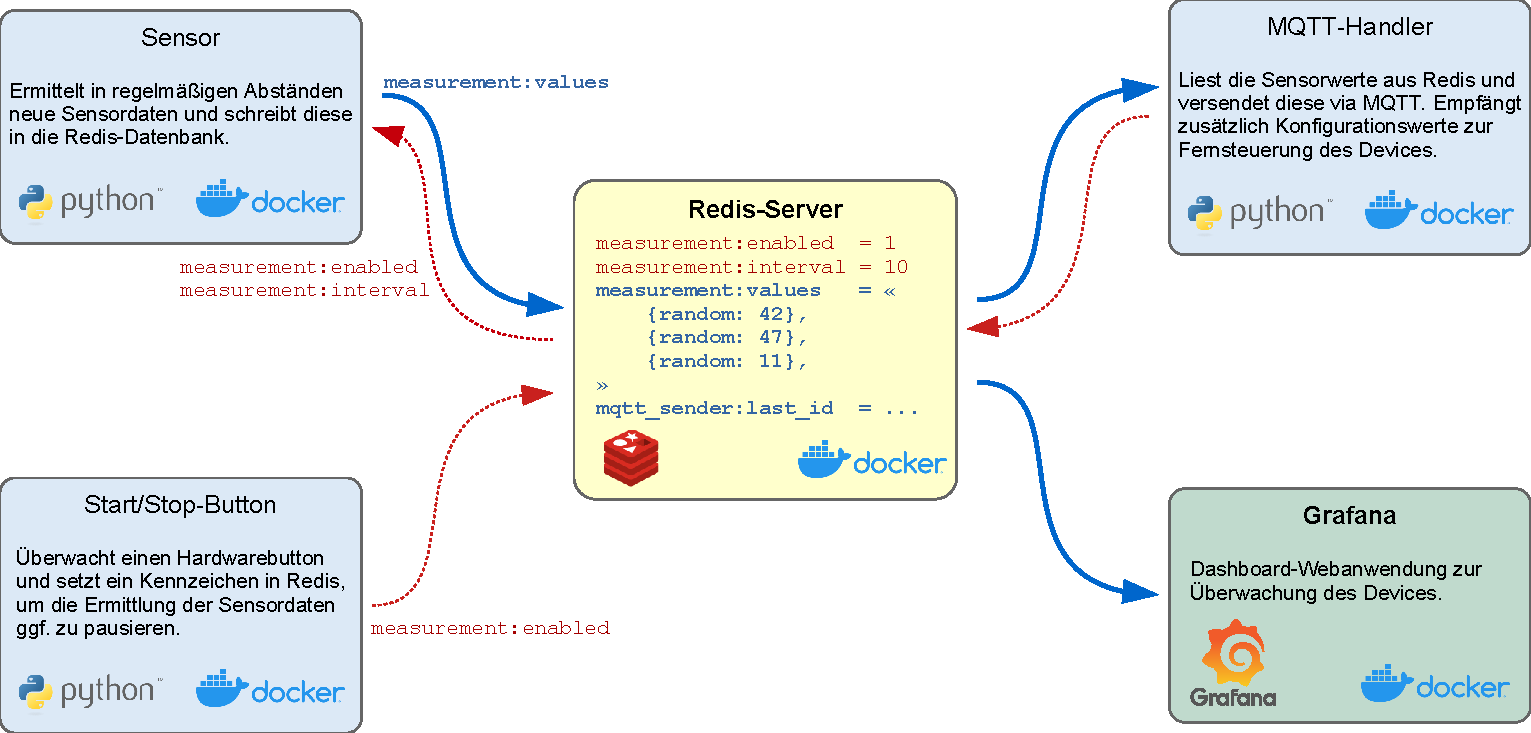
\includegraphics[width=\textwidth]{06-architektur/img/redis3}
    \end{center}

    \bigskip

    \Justified{
        \tiny
        Die obige Abbildung zeigt, wie der auf dem Pi installierte Redis-Server
        von den deviceseitigen Anwendungskomponenten genutzt wird, um sich zu
        koordinieren. Im Wesentlichen schreibt das Sensor-Programm einen Strom
        (in Redis ,,Stream'' genannt) strukturierter Sensordaten, der vom
        MQTT-Handler und dem Grafana-Dashboard in Echtzeit überwacht wird, um
        diese in das Internet zu versenden bzw. einem lokal installierten
        Web-Dashboard darzustellen. Über den MQTT-Handler könnten darüber hinaus
        Konfigurationswerte empfangen werden, die als atomare Werte in Redis
        abgelegt werden. Sie werden vom Sensorprogramm ausgewertet sowie vom
        Start/Stop-Programm verändert, wenn der Anwender einen an den Pi
        angeschlossenen Knopf zum Unterbrechen der Messungen drückt.
    }
\end{frame}

%%% Folie
\begin{frame}[allowframebreaks]{Aufgabe: Redis Tutorial}
    \setlength{\fboxsep}{0em}
    \fbox{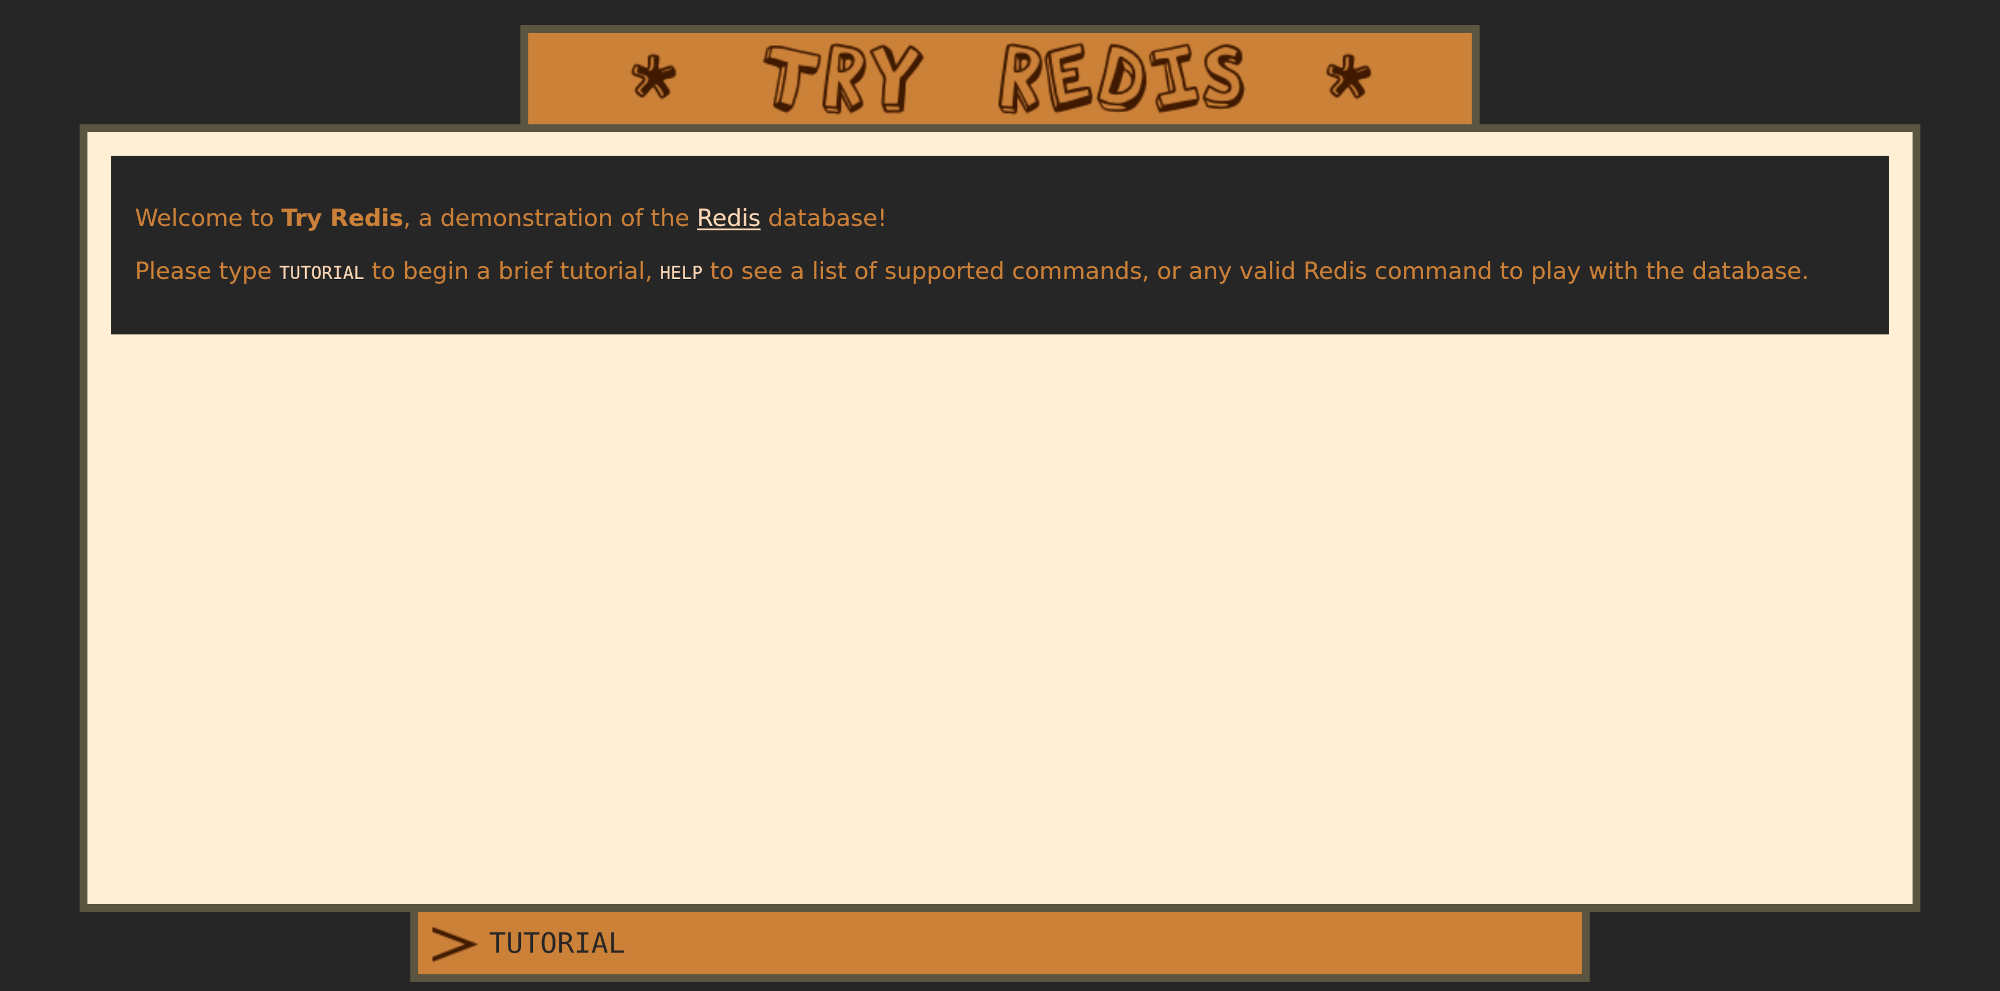
\includegraphics[width=\linewidth]{06-architektur/img/redis-tutorial}}

    Bearbeiten Sie das Redis Tutorial auf \url{https://try.redis.io/}.

    \framebreak

    {
        \footnotesize
        Beantworten Sie nun die folgenden Fragen zum Tutorial:
    }
    \bigskip
    {
    \scriptsize

    \begin{enumerate}
        \item Mit welchen Befehlen können atomare Werte geschrieben oder gelesen werden?
        \item Mit welchem Befehl kann die Existenz eines Werts überprüft werden?
        \item Wie können atomare Zähler in Redis realisiert werden?
        \item Wie lösen atomare Zähler in Redis das Lost-Update-Problem?
        \item Wie kann die Lebensdauer eines Werts begrenzt werden?
        \item Wie kann die Lebensdauer eines Werts geprüft werden?
        \item Wie kann die Begrenzung wieder aufgehoben werden?
        \item Mit welchen Befehlen können Listen in Redis manipuliert werden?
        \item Wie kann ein Wert vom Anfang oder Ende einer List entnommen werden?
        \item Was ist der Unterschied zwischen einer Liste und einer Menge (Set)?
        \item Überlegen Sie sich einen Anwendungsfall für Mengen in Redis.
        \item Wie kann einer sortierte Liste in Redis definiert werden?
        \item Nach welchen Kriterien wird die Liste sortiert?
        \item Was ist ein Hash Field in Redis und welchem Python-Typ kommt es am nächsten?
        \item Zeigen Sie ein Beispiel zur Verwendung von Hash Fields in Redis.
    \end{enumerate}
    }
\end{frame}

%-------------------------------------------------------------------------------
\section{Datenaustausch mit MQTT}
%-------------------------------------------------------------------------------

%%% Folie
\begin{frame}[fragile]{Das Problem synchroner Punkt-zu-Punkt-Verbindungen}
    \only<beamer:1|handout:0>{
        \begin{tikzpicture}[remember picture,overlay]
            \node at (5.4cm,0.28cm){
                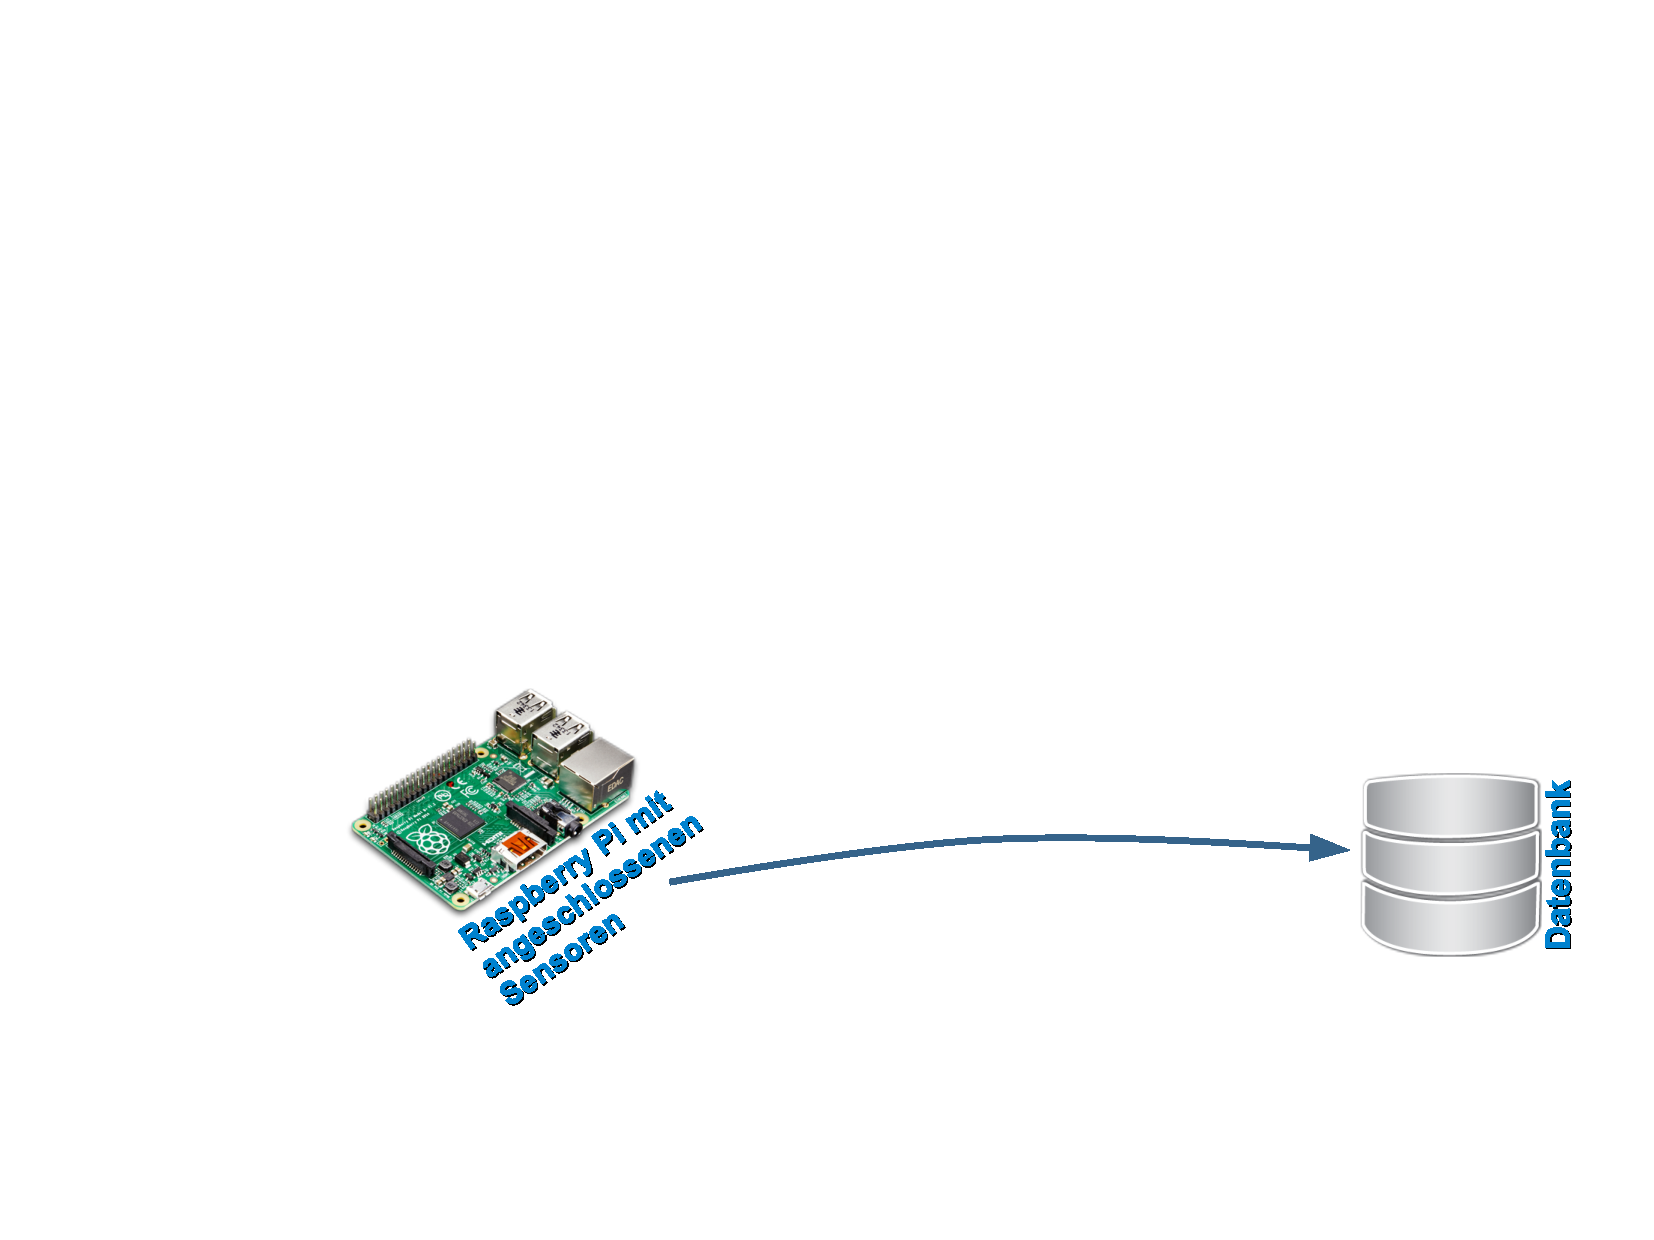
\includegraphics[width=\linewidth]{06-architektur/img/mqtt1}
            };
        \end{tikzpicture}
    }

    \only<beamer:2|handout:0>{
        \transdissolve

        \begin{tikzpicture}[remember picture,overlay]
            \node at (5.4cm,0.28cm){
                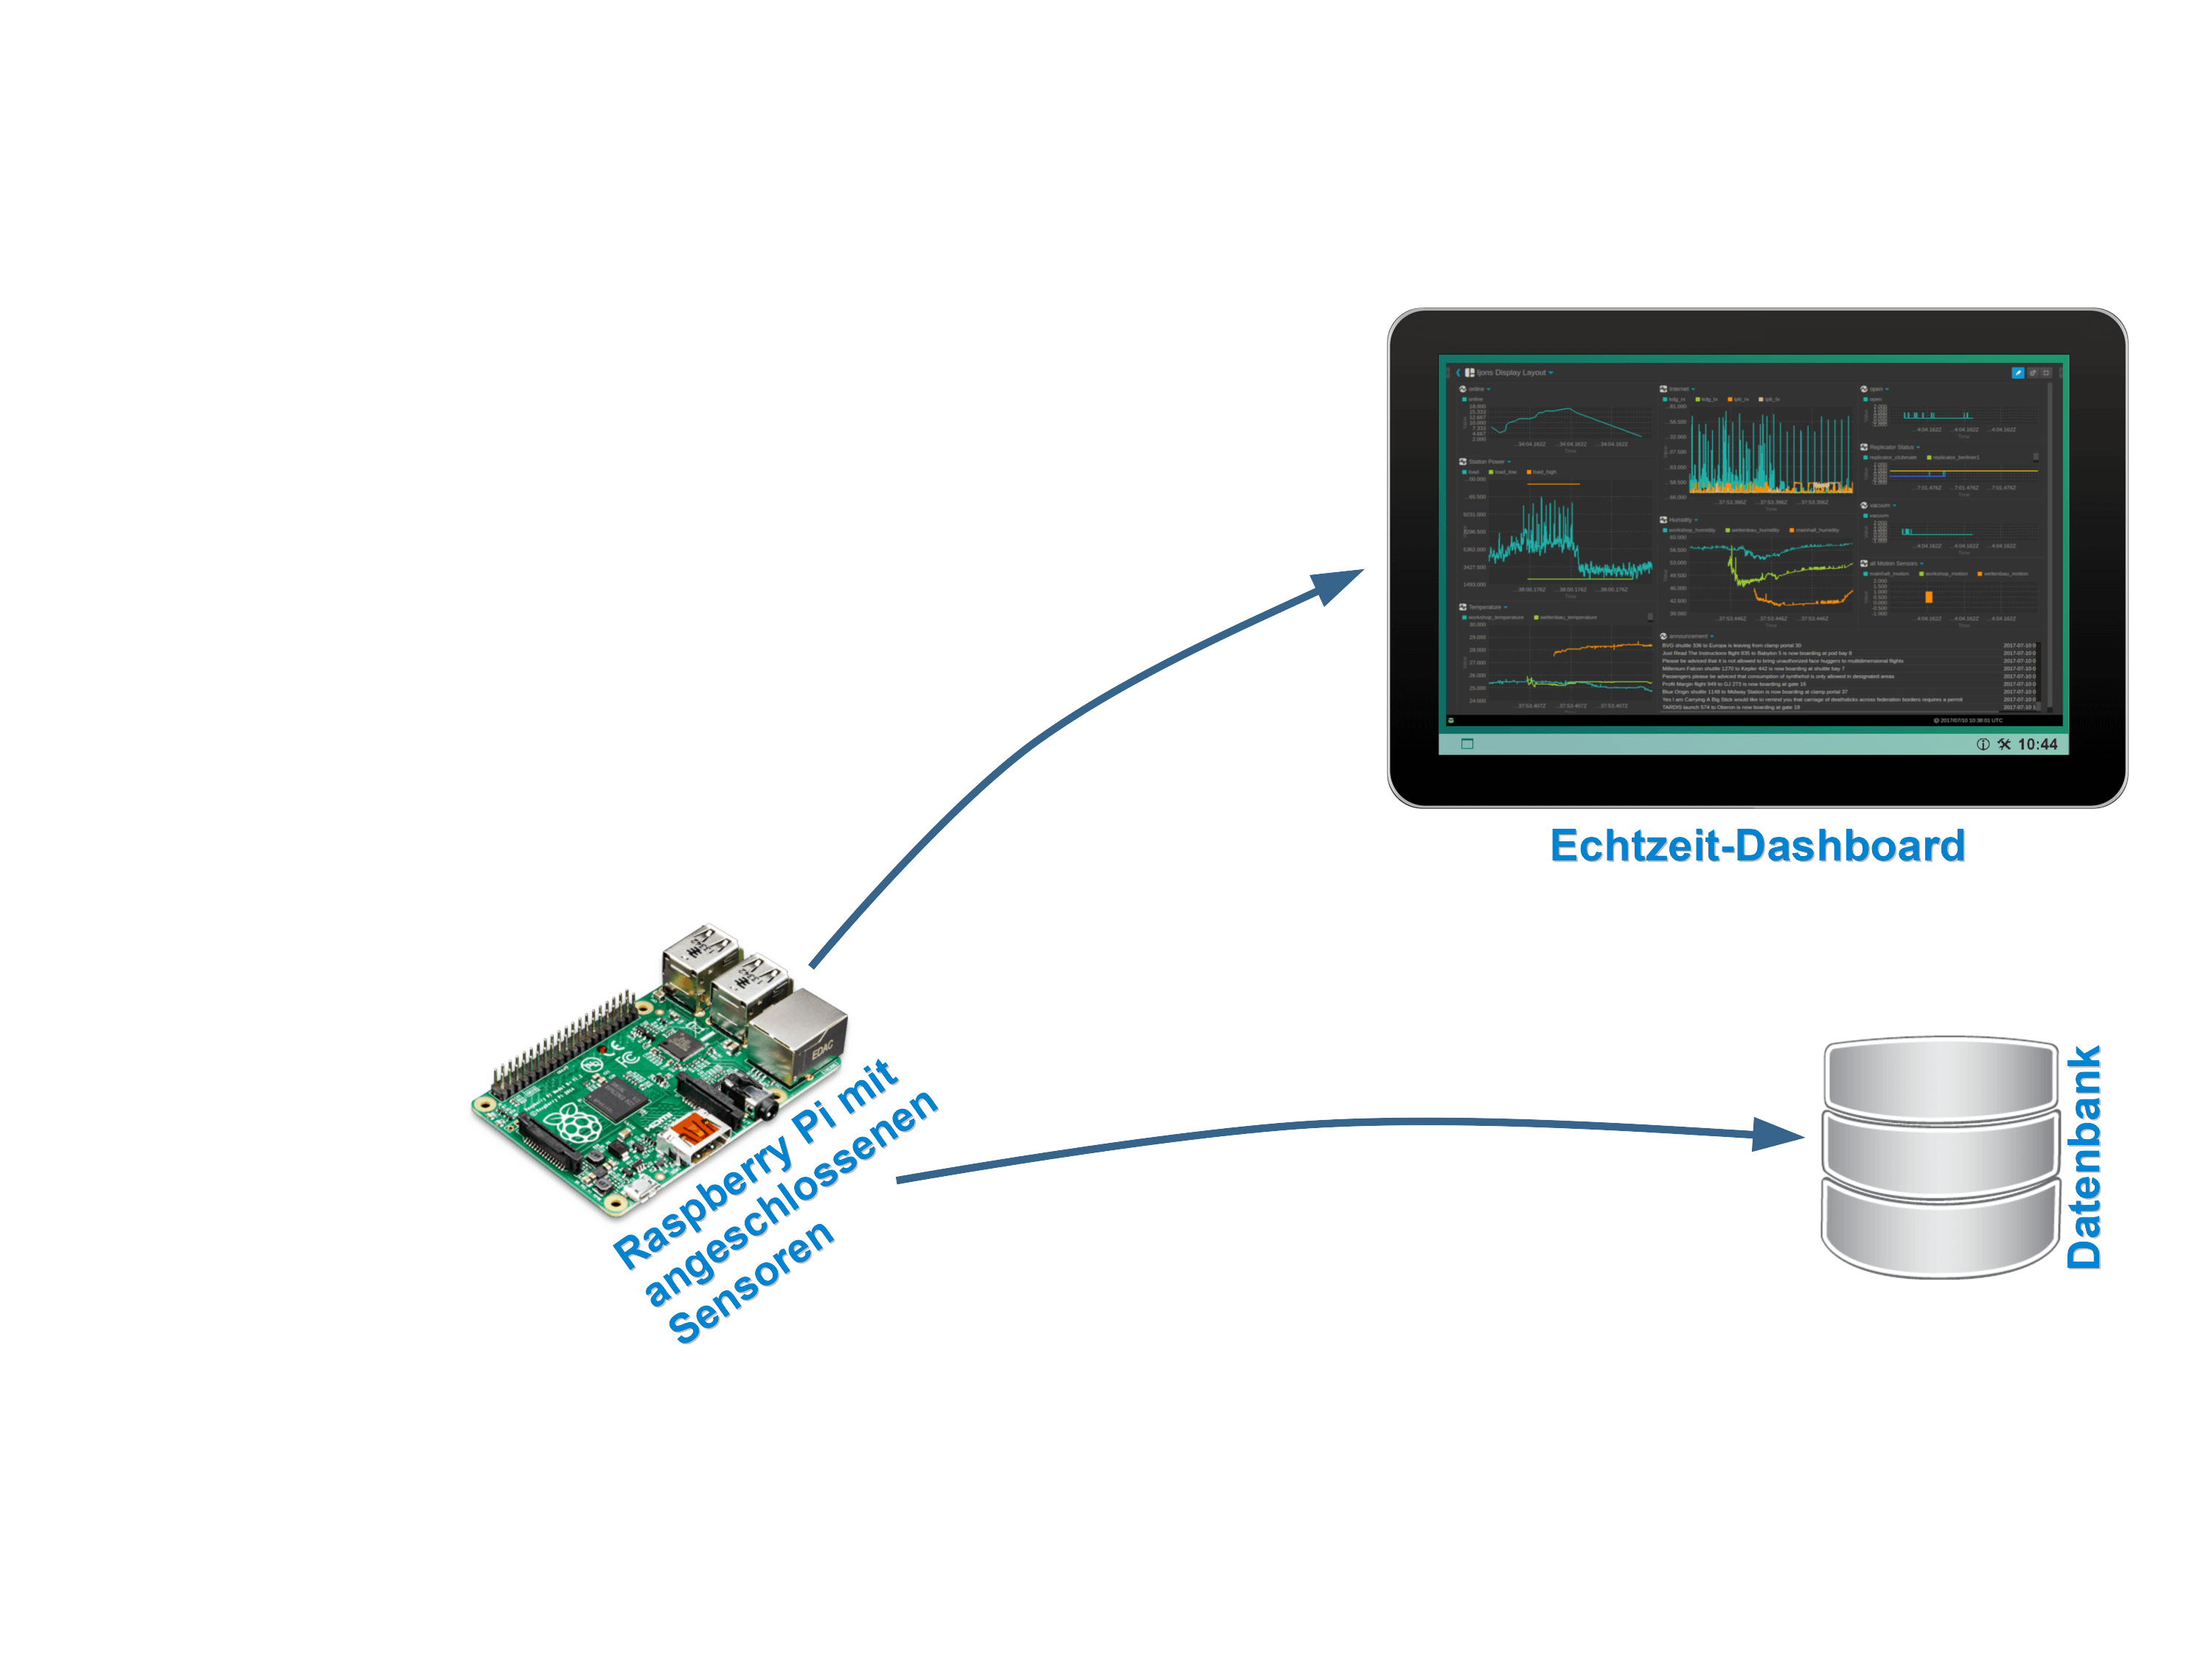
\includegraphics[width=\linewidth]{06-architektur/img/mqtt2}
            };
        \end{tikzpicture}
    }

    \only<beamer:3|handout:1>{
        \transdissolve

        \begin{tikzpicture}[remember picture,overlay]
            \node at (5.4cm,0.28cm){
                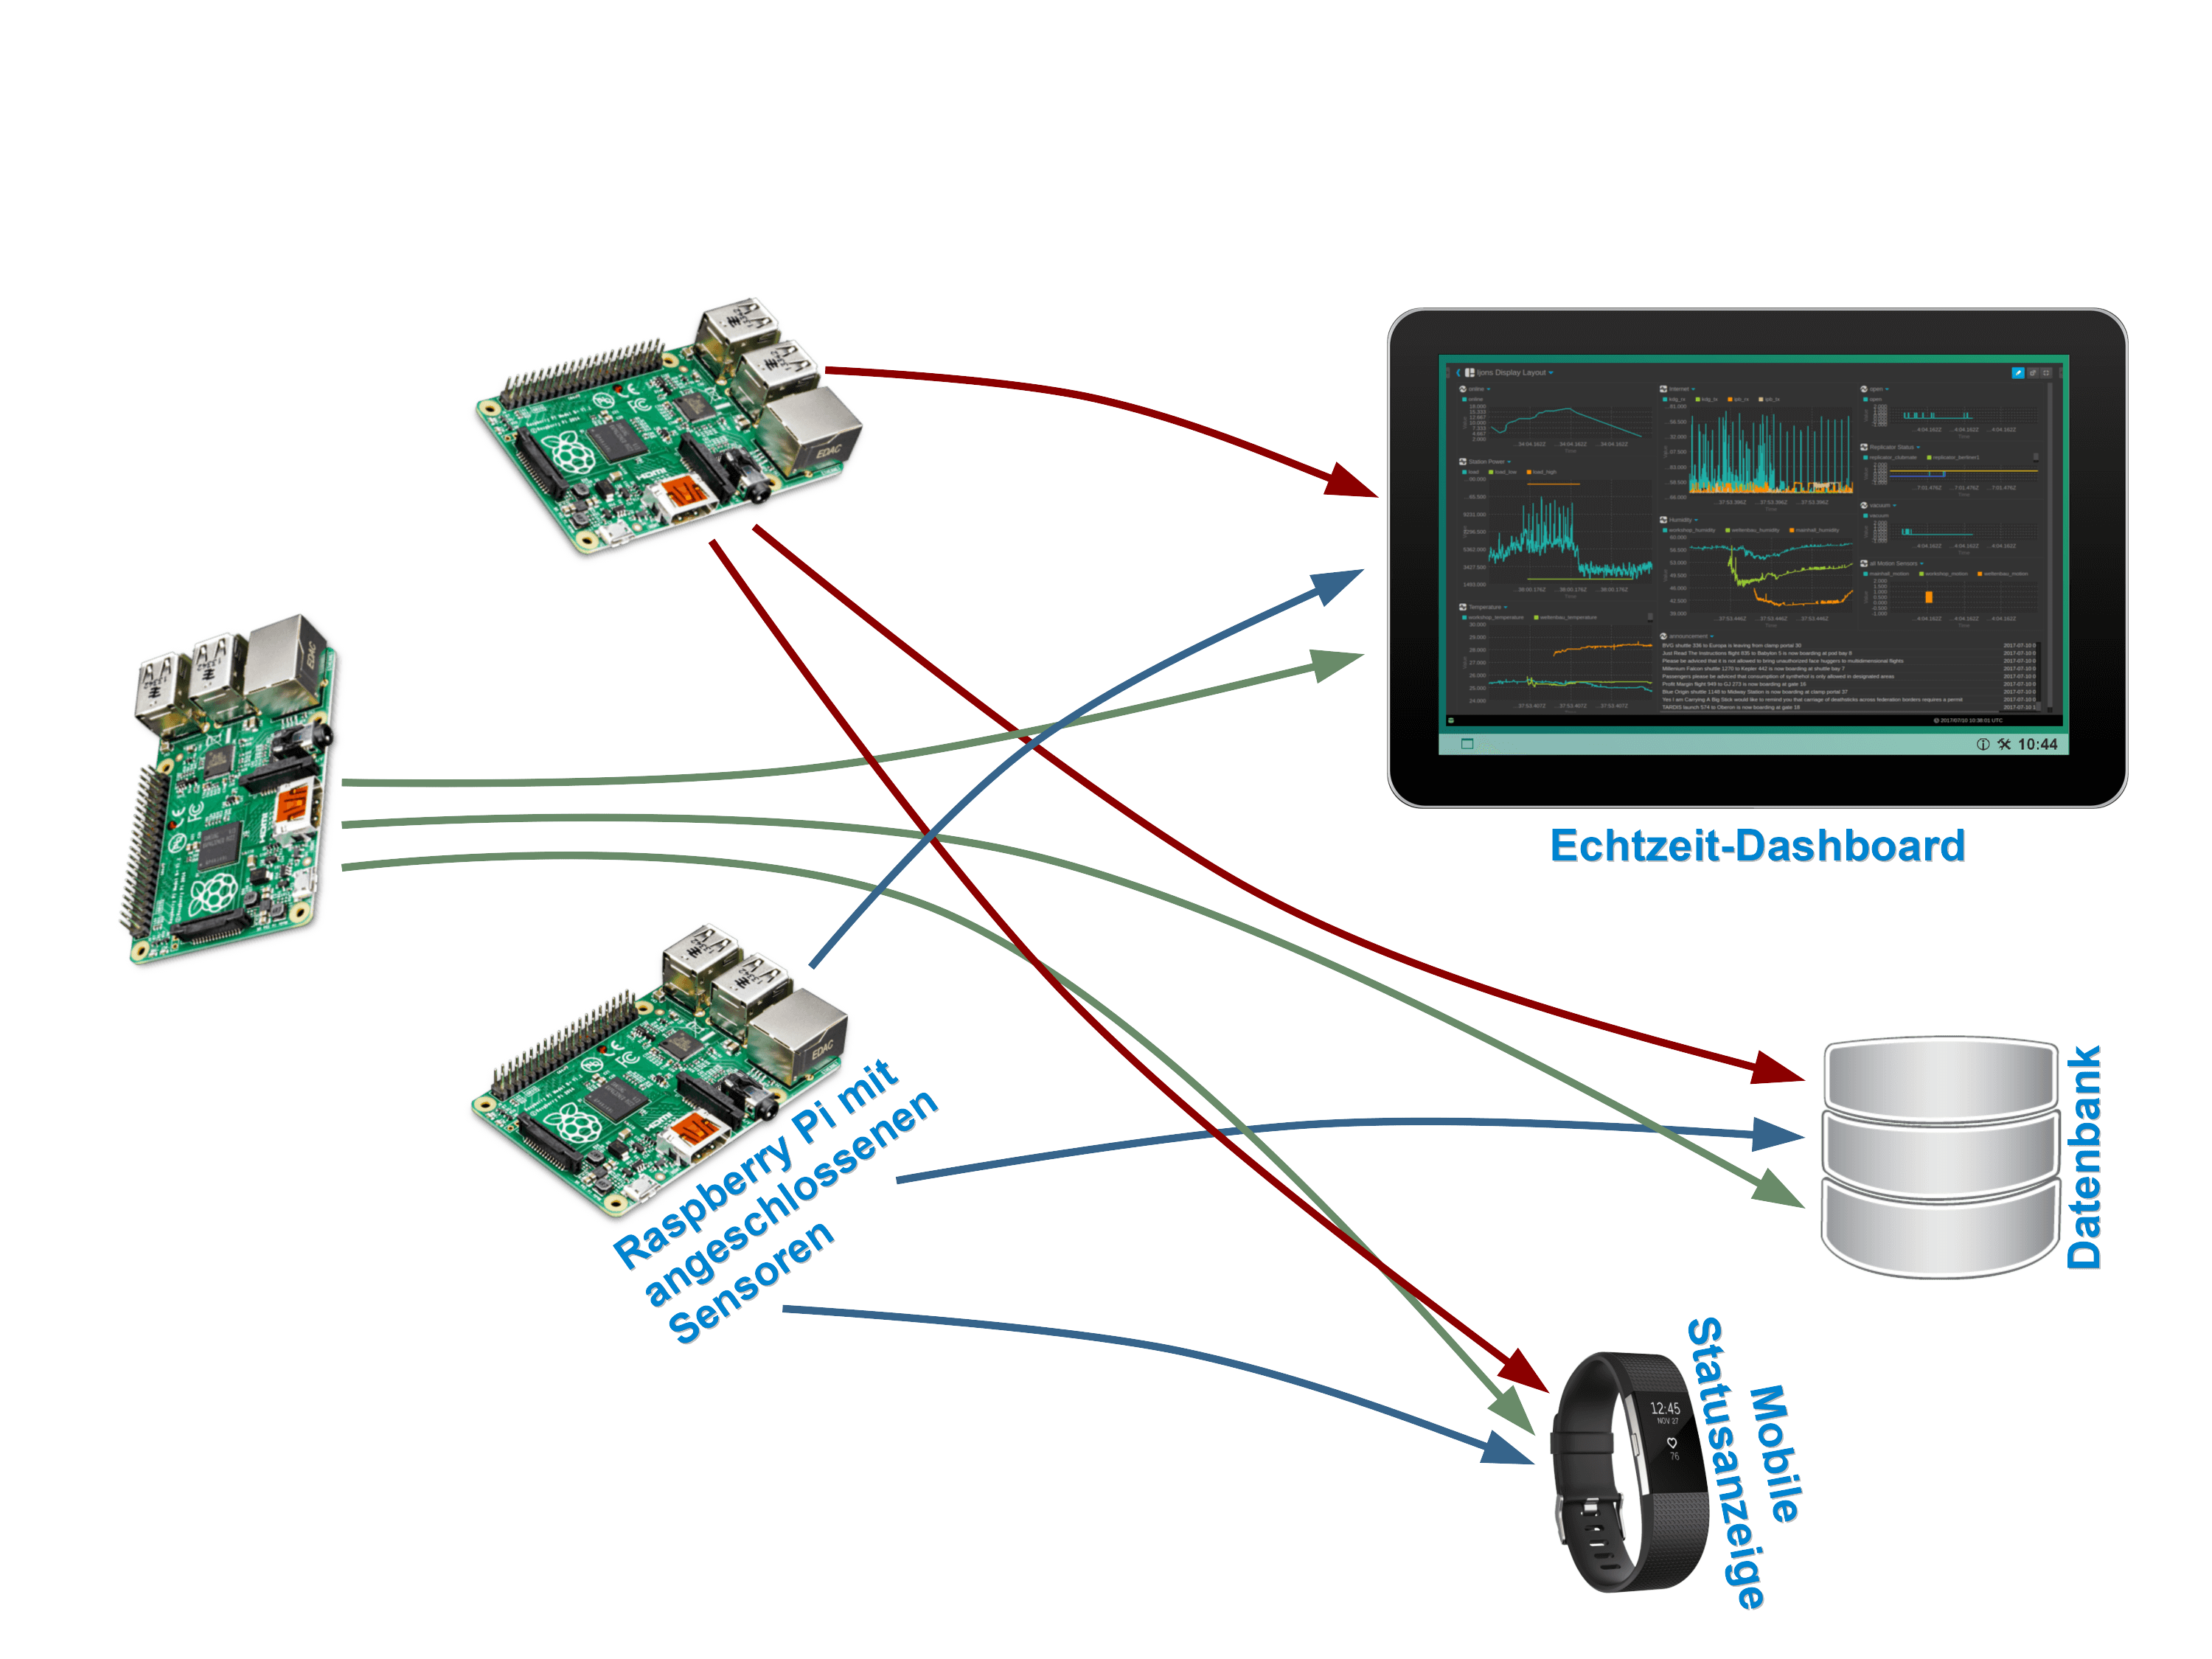
\includegraphics[width=\linewidth]{06-architektur/img/mqtt3}
            };
        \end{tikzpicture}
    }
\end{frame}

\begin{frame}{Zunehmende Komplexität bei P2P}
    \begin{center}
        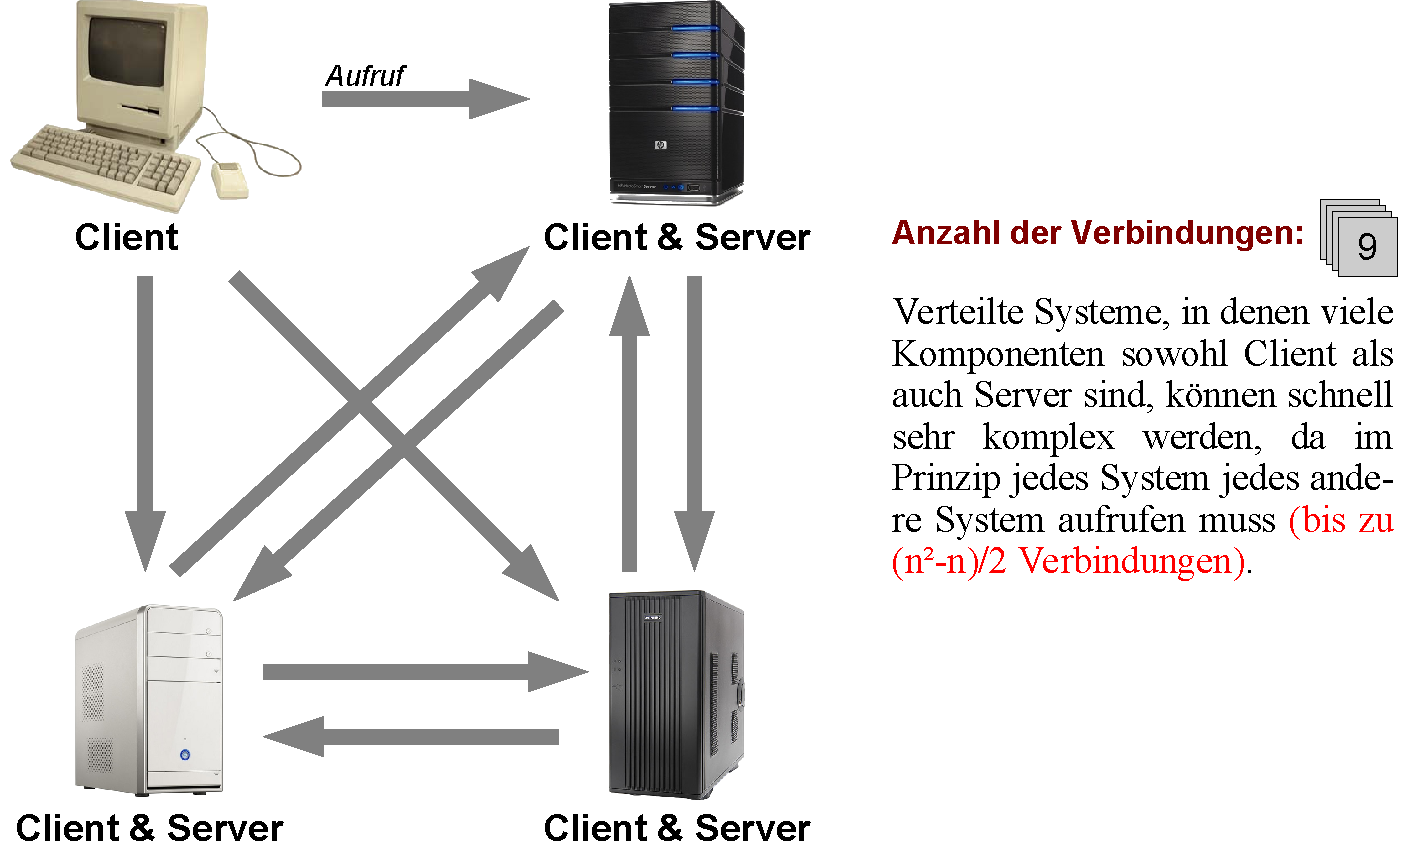
\includegraphics[width=\linewidth]{06-architektur/img/mqtt4}
    \end{center}
\end{frame}

\begin{frame}{Lösung durch einen zentralen Message Broker}
    \begin{center}
        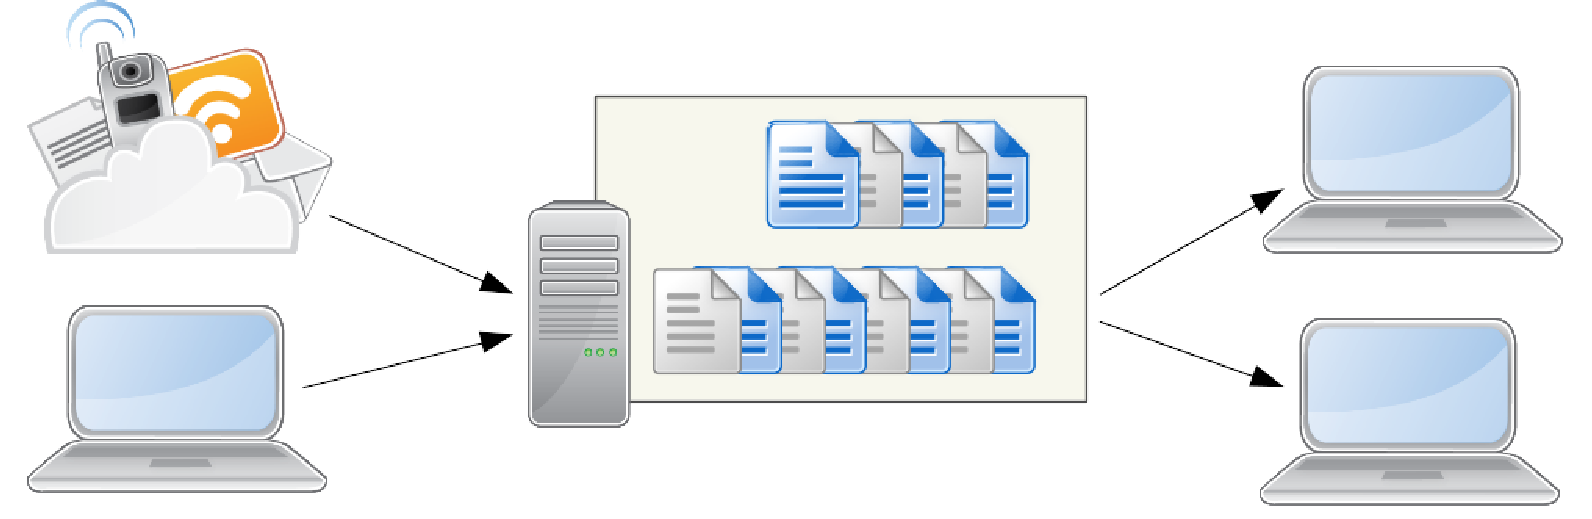
\includegraphics[width=\linewidth]{06-architektur/img/mqtt5}
    \end{center}
\end{frame}

\begin{frame}{Das Publish/Subscribe-Verfahren bei MQTT}
    \begin{center}
        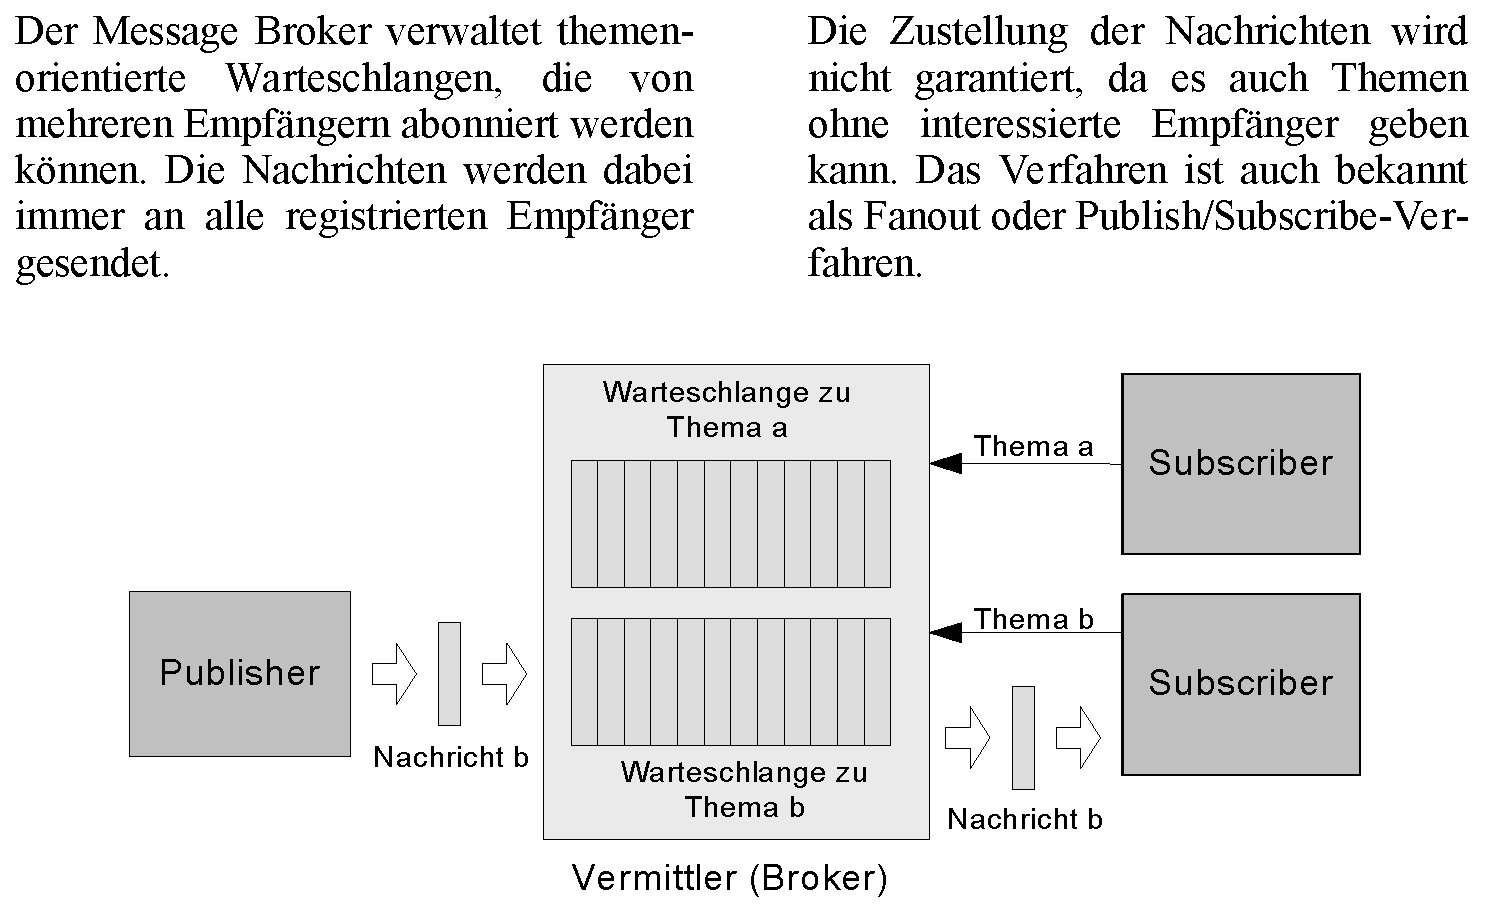
\includegraphics[width=\linewidth]{06-architektur/img/mqtt6}
    \end{center}
\end{frame}

\begin{frame}{Simulation des synchronen Request/Response-Verfahrens }
    \begin{center}
        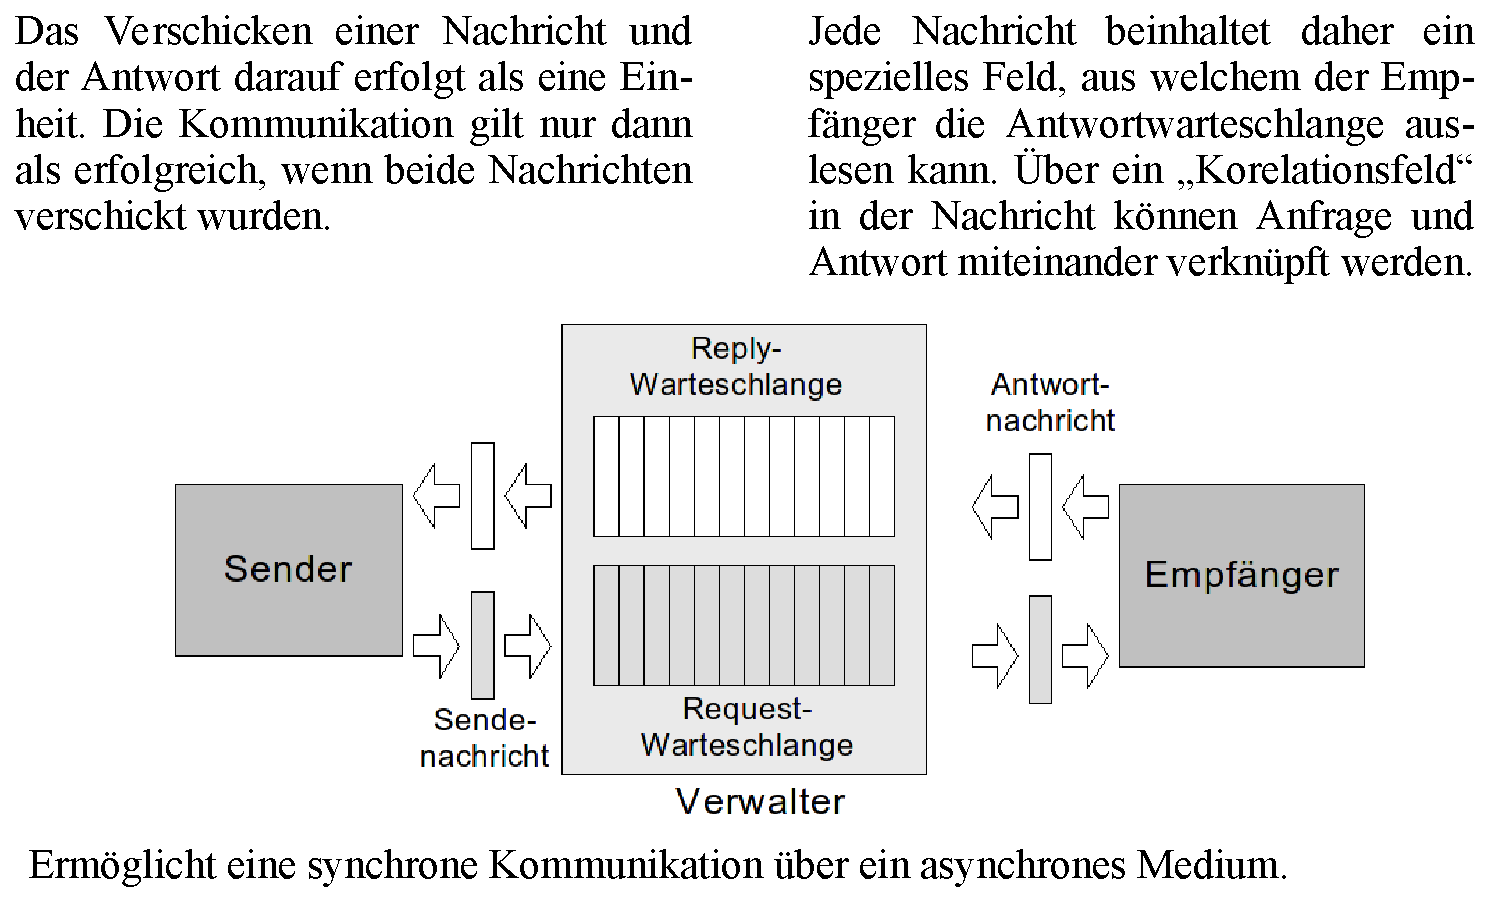
\includegraphics[width=\linewidth]{06-architektur/img/mqtt7}
    \end{center}
\end{frame}

%\begin{frame}[allowframebreaks, fragile]{Das Problem synchroner Punkt-zu-Punkt-Verbindungen}
    %\begin{center}
        %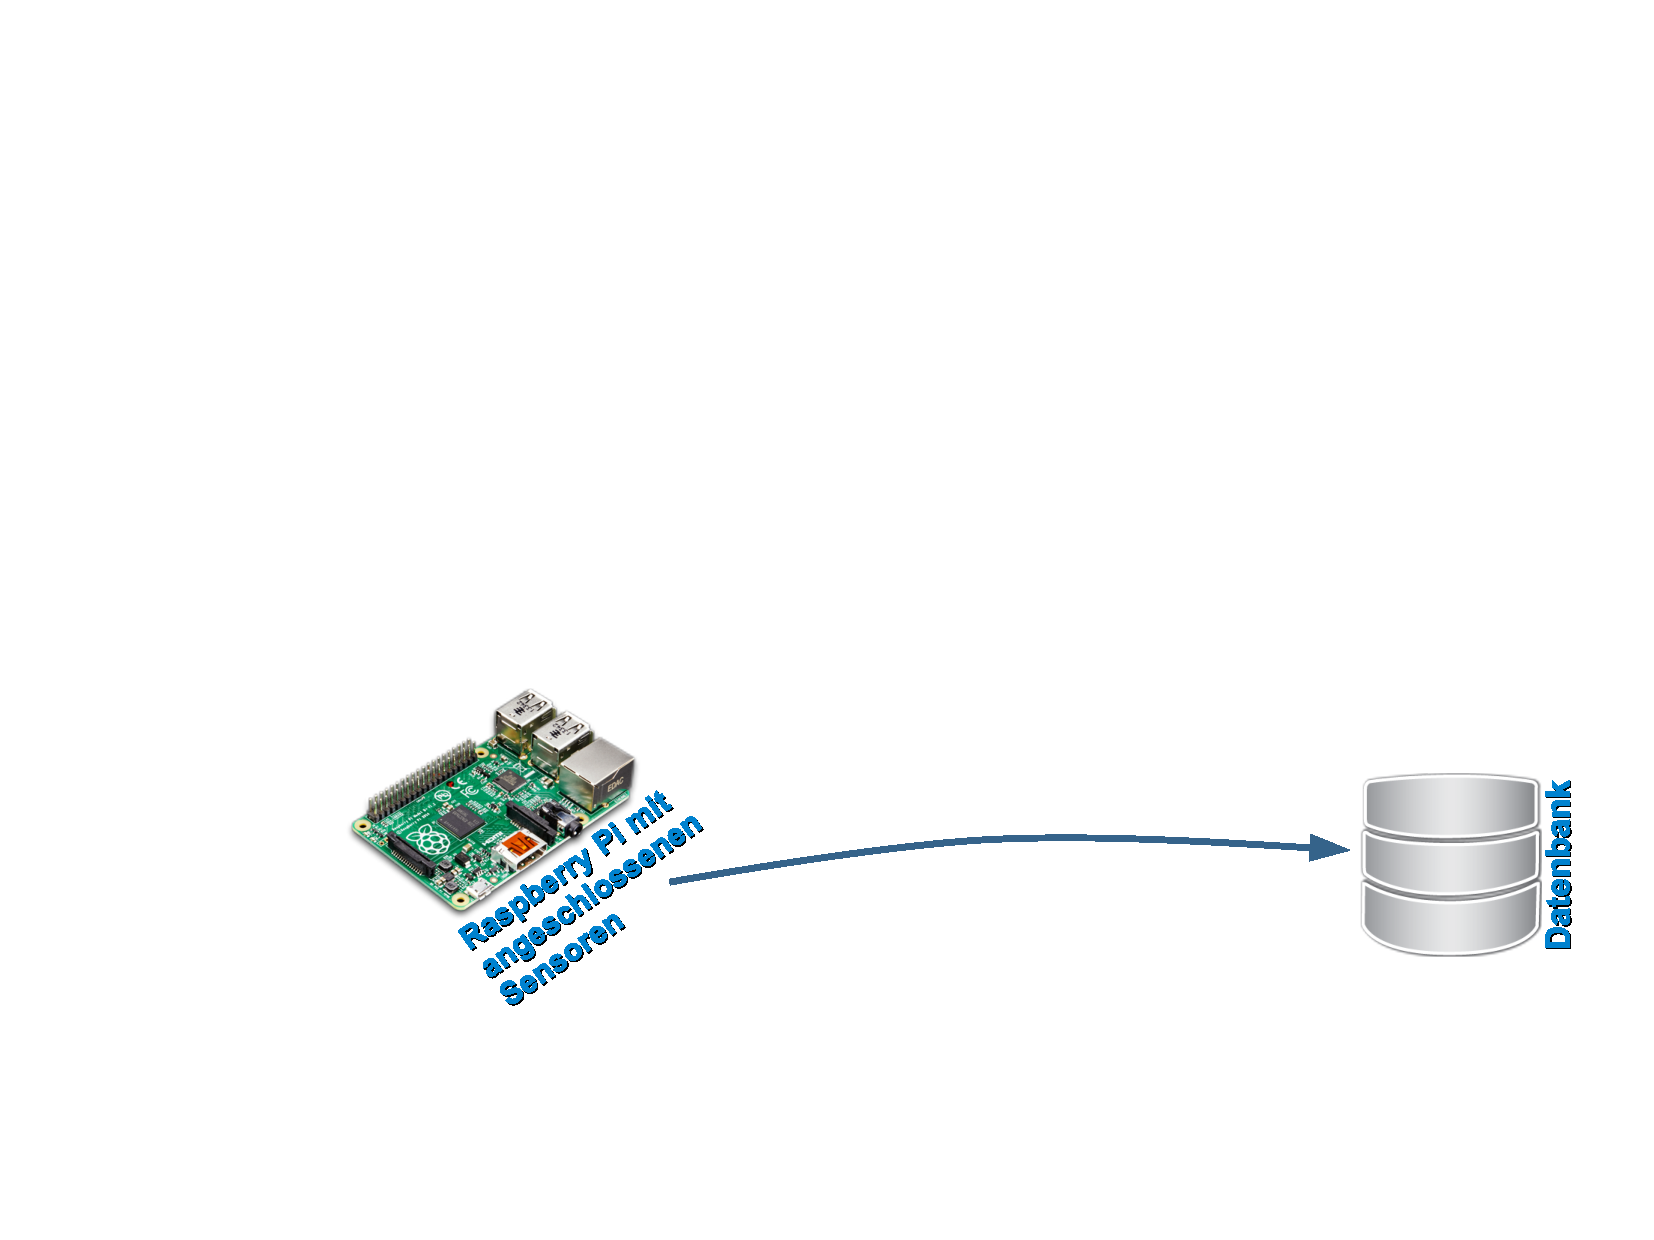
\includegraphics[width=\textwidth]{06-architektur/img/mqtt1}
    %\end{center}

    %\framebreak

    %\begin{center}
        %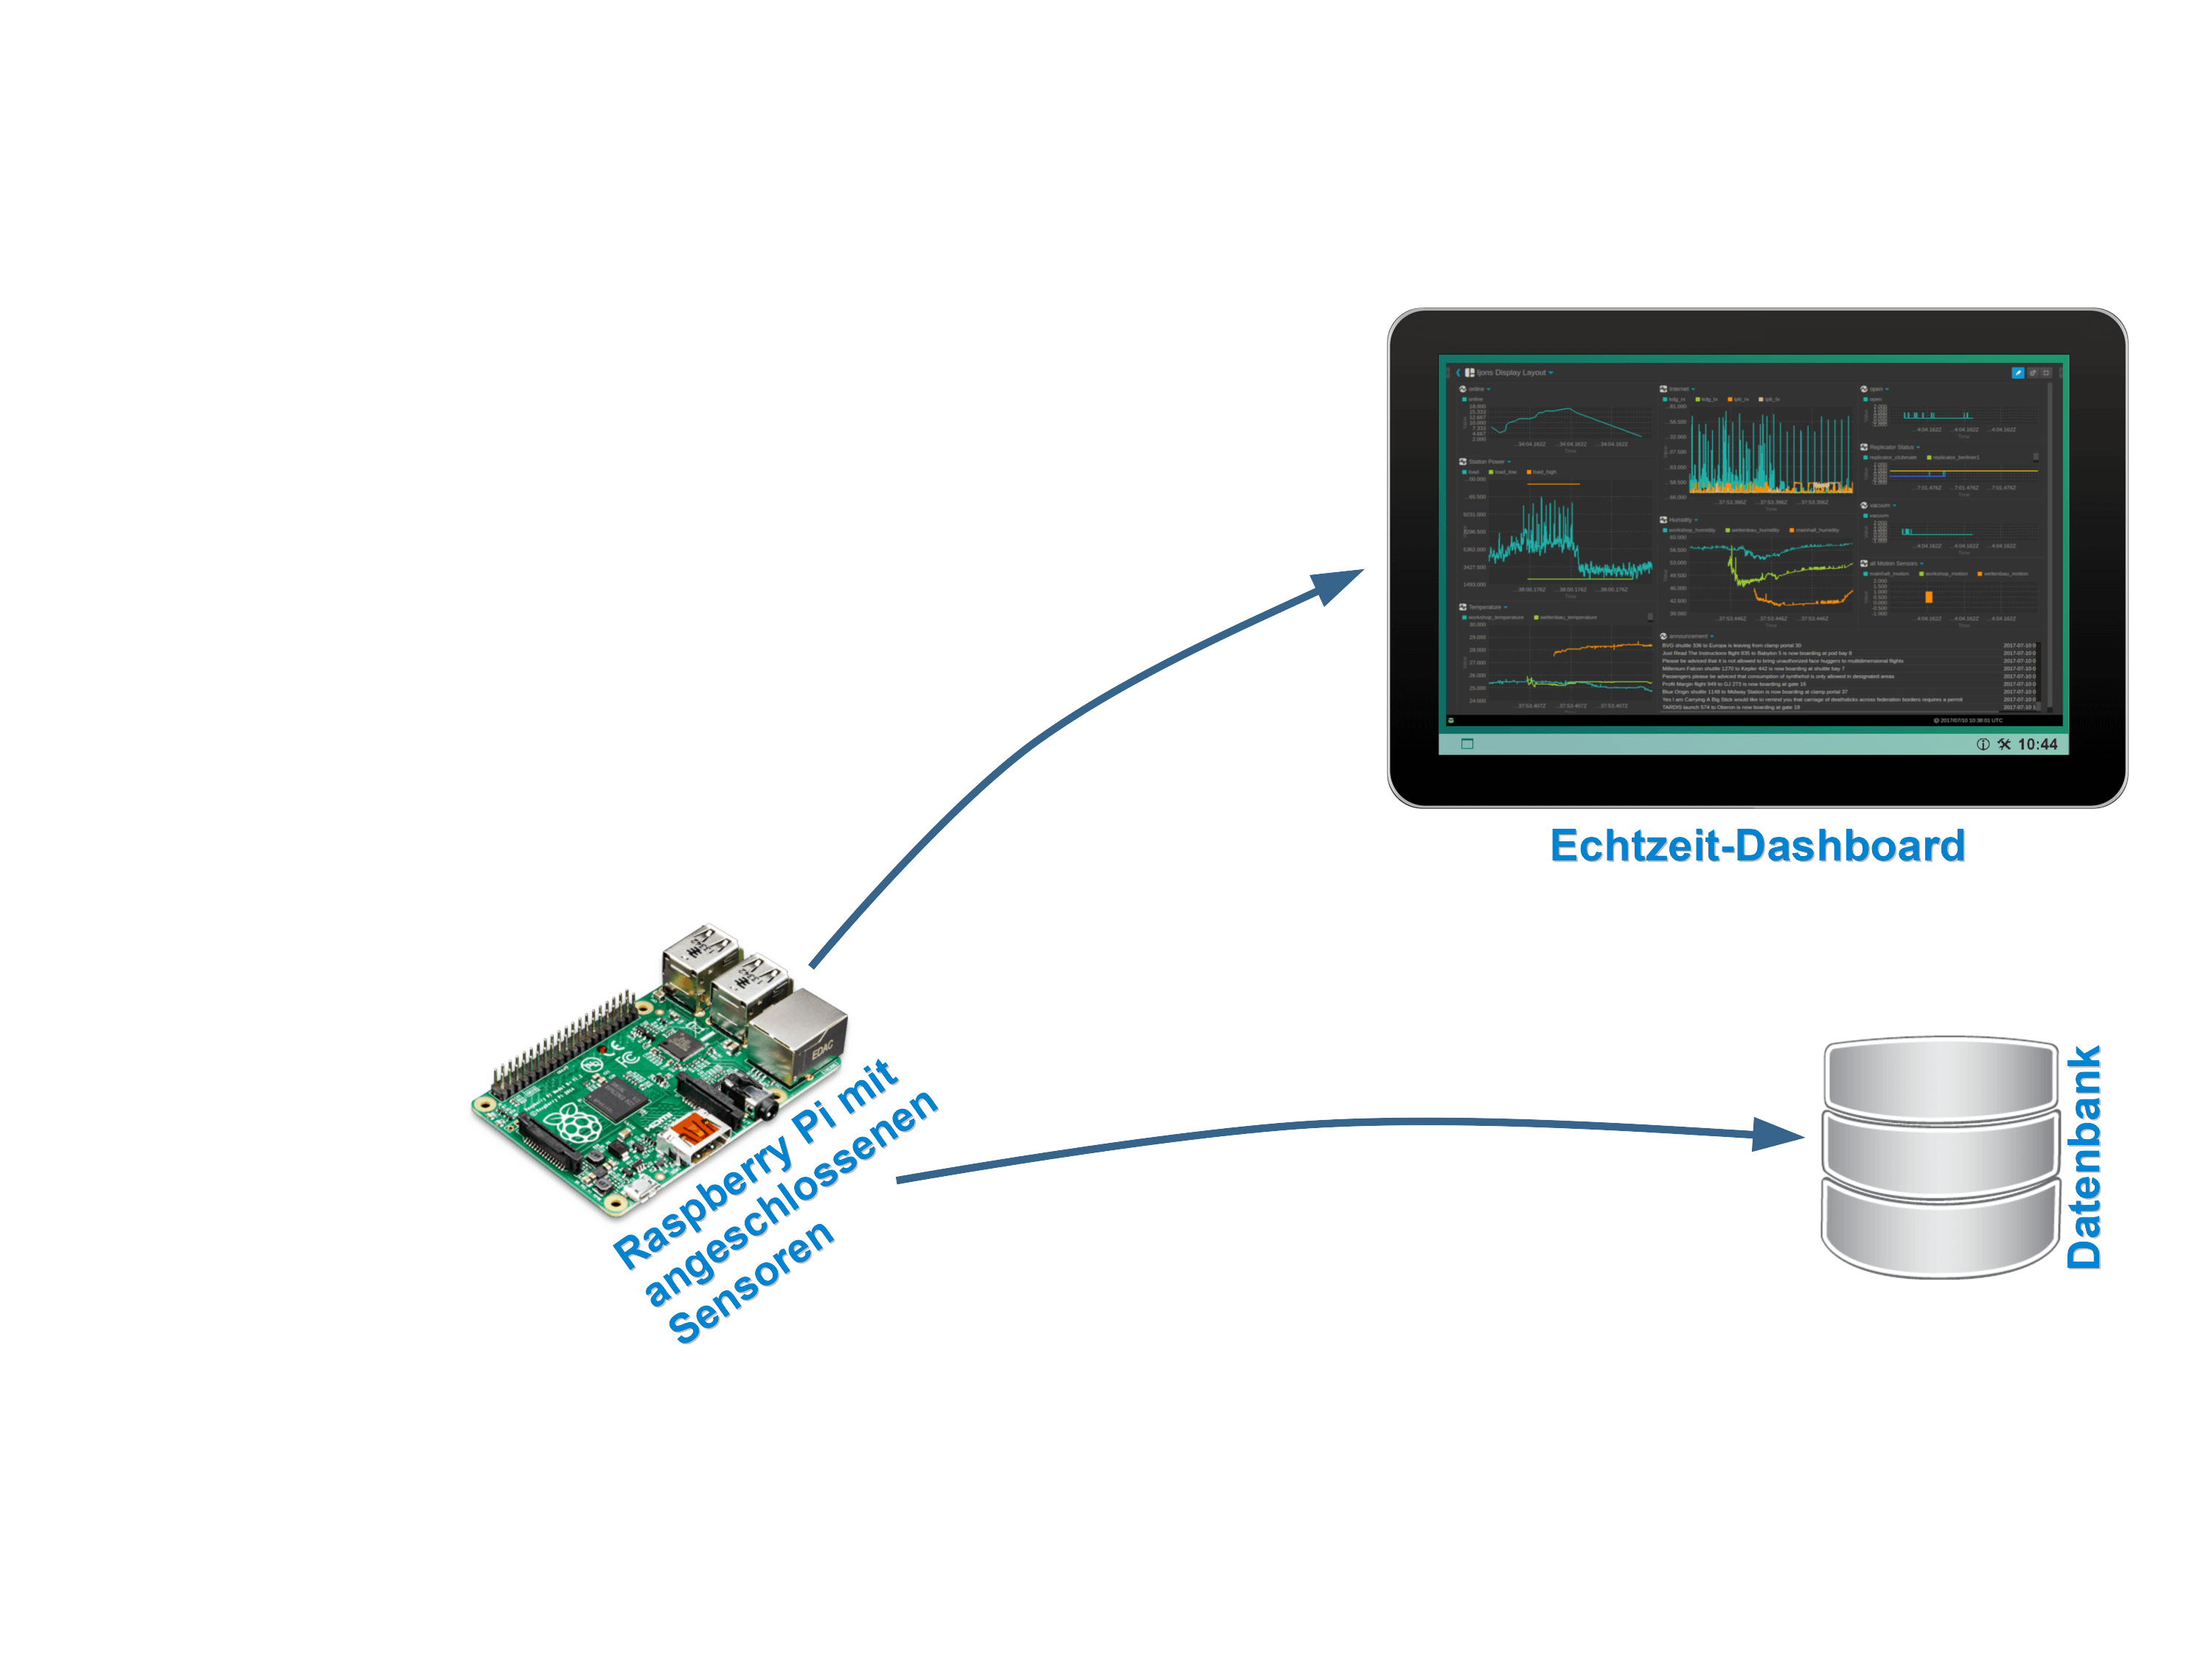
\includegraphics[width=\textwidth]{06-architektur/img/mqtt2}
    %\end{center}

    %\framebreak

    %\begin{center}
        %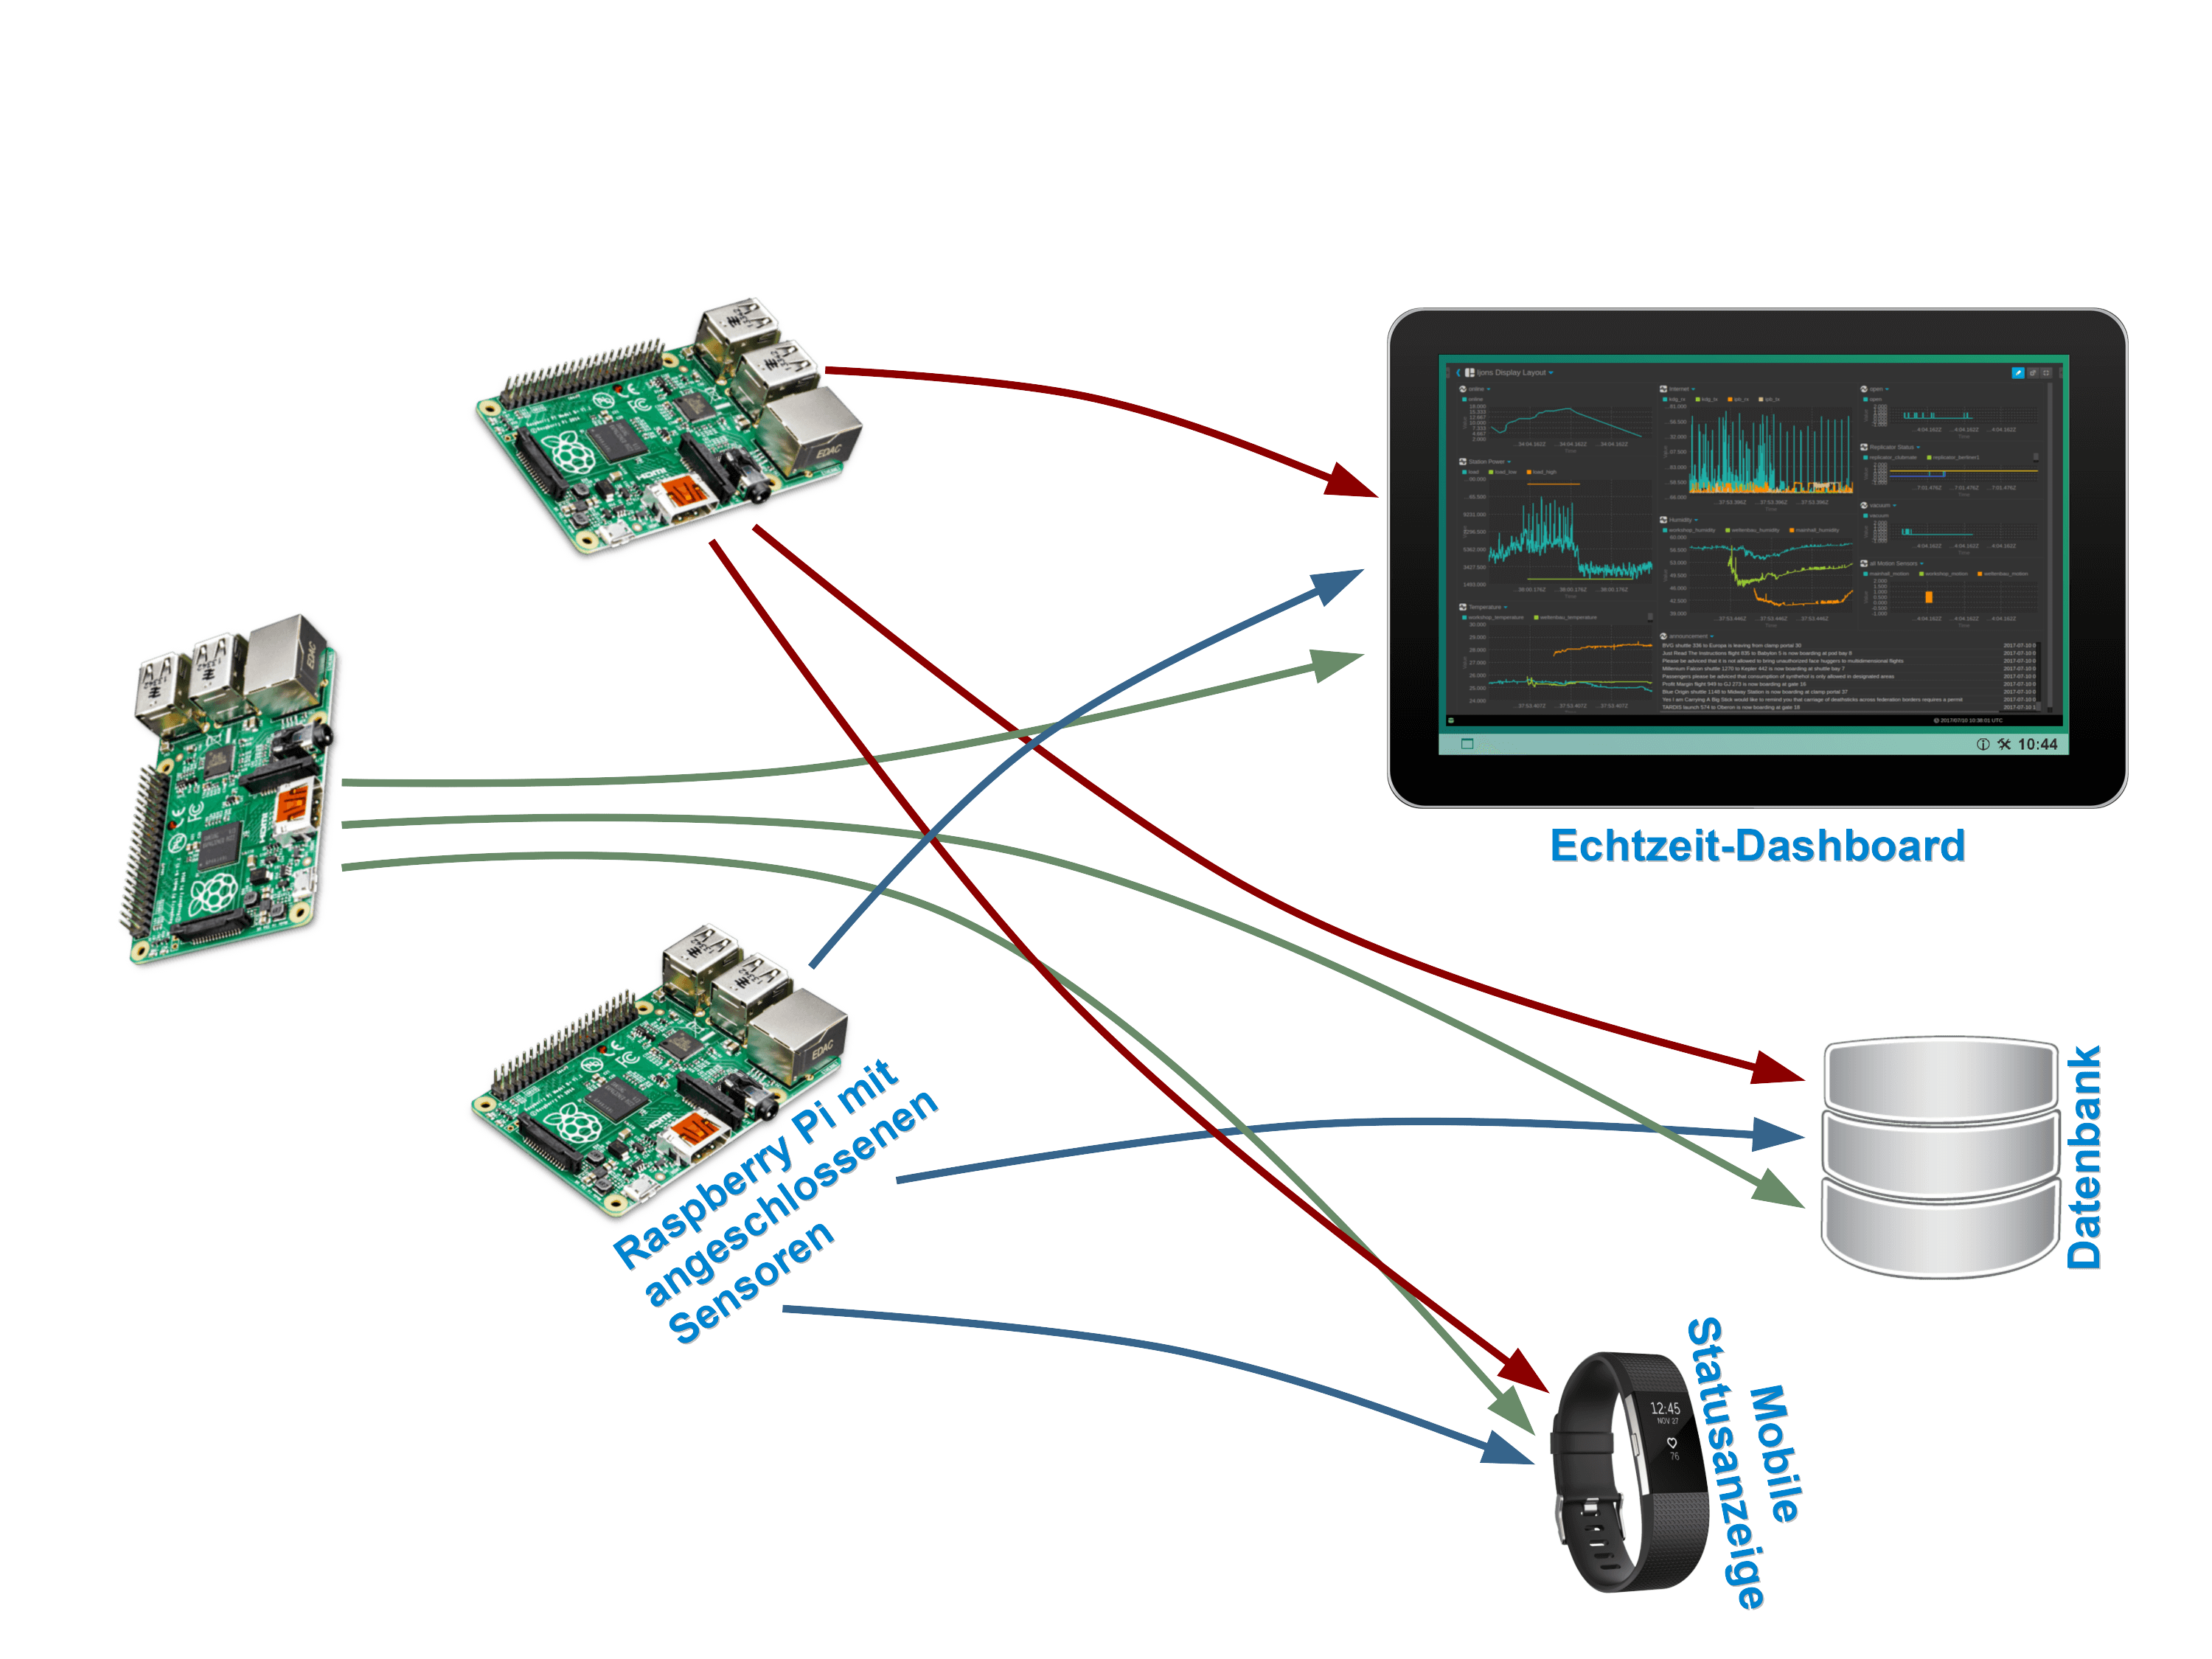
\includegraphics[width=\textwidth]{06-architektur/img/mqtt3}
    %\end{center}
%\end{frame}
